% !TEX program = xelatex
\documentclass[UTF8,fontset=fandol,a4paper,11pt]{ctexart}
\usepackage[margin=21mm,top=23mm,bottom=22mm,headheight=16pt]{geometry}
\usepackage{amsmath,amssymb,mathtools,bm}
\usepackage{tikz}
\usetikzlibrary{arrows.meta,calc,angles,quotes,patterns}
\usepackage{xcolor,booktabs,array,longtable,enumitem,fancyhdr,needspace}
\usepackage[unicode,hidelinks]{hyperref}
\definecolor{ink}{HTML}{24343C}
\definecolor{accent}{HTML}{166A70}
\definecolor{muted}{HTML}{65747A}
\definecolor{rulegray}{HTML}{D4DDE0}
\definecolor{warm}{HTML}{966037}
\color{ink}
\setlength{\parindent}{2em}
\setlength{\parskip}{4pt}
\linespread{1.12}
\AtBeginDocument{\setlength{\abovedisplayskip}{6pt plus 2pt minus 1pt}
\setlength{\belowdisplayskip}{6pt plus 2pt minus 1pt}
\setlength{\abovedisplayshortskip}{0pt plus 1pt}
\setlength{\belowdisplayshortskip}{4pt plus 1pt}}
\setlist[enumerate]{label=(\arabic*),leftmargin=2.3em,itemsep=3pt,topsep=4pt}
\setlist[itemize]{leftmargin=2em,itemsep=2pt,topsep=4pt}
\allowdisplaybreaks[1]
\setlength{\emergencystretch}{2em}
\setcounter{secnumdepth}{0}
\providecommand{\tightlist}{\setlength{\itemsep}{0pt}\setlength{\parskip}{0pt}}
\ctexset{section={format=\Large\bfseries\color{accent},beforeskip=10pt,afterskip=9pt},
subsection={format=\normalsize\bfseries\color{accent},beforeskip=10pt,afterskip=4pt},
subsubsection={format=\normalsize\bfseries,beforeskip=8pt,afterskip=3pt}}
\pagestyle{fancy}
\fancyhf{}
\fancyhead[L]{\small\color{muted}物理学难题集萃}
% 页眉仅保留书名；版本名称只在封面显示。
\fancyfoot[L]{\small\color{muted}\chapterlabel}
\fancyfoot[R]{\small\thepage}
\renewcommand{\headrulewidth}{0.4pt}
\renewcommand{\footrulewidth}{0pt}
\newcommand{\dd}{\mathop{}\!\mathrm{d}}
\newcommand{\vect}[1]{\bm{#1}}
\newcommand{\tagline}[1]{\noindent{\small\color{muted}#1}\par}
\newcommand{\result}[1]{\begin{equation*}\boxed{#1}\end{equation*}}
\newcommand{\figcaption}[1]{\par\vspace{2pt}{\small\color{muted}#1}\par}
\newcommand{\teach}[2]{\Needspace{4\baselineskip}\subsection*{讲解要点与追问}#1\par\smallskip\noindent\textbf{追问：}#2\par}
\newcommand{\workarea}{\par\vspace{7mm}\noindent{\small\color{muted}作答区}\par\vspace{4mm}
\noindent\textcolor{rulegray}{\rule{\linewidth}{0.3pt}}\par\vspace{16mm}
\noindent\textcolor{rulegray}{\rule{\linewidth}{0.3pt}}\par\vspace{16mm}
\noindent\textcolor{rulegray}{\rule{\linewidth}{0.3pt}}\par\vspace{16mm}
\noindent\textcolor{rulegray}{\rule{\linewidth}{0.3pt}}}
\tikzset{axis/.style={-{Stealth[length=2mm]},thin,color=muted},
motion/.style={-{Stealth[length=2.3mm]},thick,color=accent},
force/.style={-{Stealth[length=2.3mm]},thick,color=warm},
traj/.style={thick,color=accent},guide/.style={dashed,thin,color=muted},
object/.style={thick,color=ink},every node/.style={font=\small}}\widowpenalty=10000\clubpenalty=10000\displaywidowpenalty=10000\newcommand{\chapterlabel}{电磁学试题（四）}







\hypersetup{pdftitle={电磁学试题（四）·学生解答版},pdfauthor={}}

\begin{document}\pdfbookmark[0]{电磁学试题（四）}{cover}

\thispagestyle{empty}\vspace*{22mm}

\noindent{\Huge\bfseries 物理学难题集萃}\par\vspace{12mm}

\noindent{\LARGE 电磁学试题（四）}\par\vspace{12mm}

\noindent{\Large\color{accent}学生解答版}\par\vspace{9mm}

\noindent\textcolor{accent}{\rule{\linewidth}{1pt}}\par\vspace{9mm}

\noindent 第1--5题\par\vfill\clearpage

\pdfbookmark[1]{题目目录}{contents}\section*{题目目录}

\begin{longtable}{@{}r p{113mm} r@{}}\toprule 题号 & 题目 & 页码\\\midrule

\hyperref[q:1]{1} & \hyperref[q:1]{非均匀导体中的体电荷与界面电荷} & \pageref{q:1} \\

\hyperref[q:2]{2} & \hyperref[q:2]{多端等效与无限内接三角形网络} & \pageref{q:2} \\

\hyperref[q:3]{3} & \hyperref[q:3]{互补RL、RC支路的相量与初始储能} & \pageref{q:3} \\

\hyperref[q:4]{4} & \hyperref[q:4]{双行CLC网络的复阻抗和功率因数} & \pageref{q:4} \\

\hyperref[q:5]{5} & \hyperref[q:5]{导体屏蔽暂态与单频等效电容} & \pageref{q:5} \\

\bottomrule\end{longtable}

\clearpage

\pdfbookmark[2]{第 1 题 非均匀导体中的体电荷与界面电荷}{q1}

\section*{第 1 题\quad 非均匀导体中的体电荷与界面电荷}\label{q:1}


长为$L$、截面积为$S$的均匀粗细导体，沿轴线$x$的电阻率为
\[
\rho(x)=\rho_0\left|\sin\frac{2\pi x}{L}\right|,\qquad 0\le x\le L.
\]
导体两端保持电势差$V(0)-V(L)=U>0$，已达稳恒状态。采用一维导电模型，电场沿轴线，电荷关系用$\varepsilon_0$描述。
\begin{enumerate}
\item 求导体电阻和电流密度。
\item 求内部体电荷密度$\rho_e(x)$，指出带正电的区段。
\item $x=L/2$处体电荷密度发生跳变，该截面上是否存在面电荷？给出判断依据。
\end{enumerate}


\begin{center}\begin{minipage}{.98\linewidth}\centering
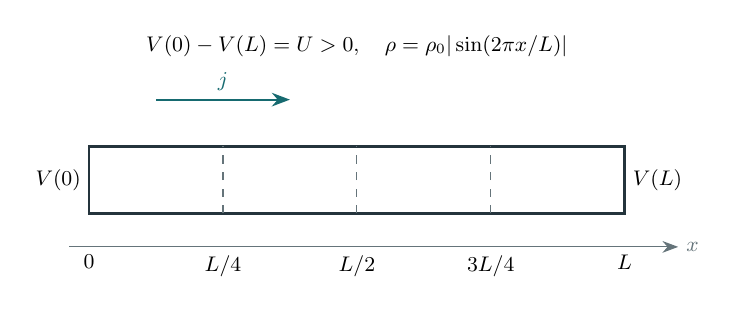
\begin{tikzpicture}[scale=.85,transform shape]

\draw[object] (0,-.5) rectangle (8,.5);
\foreach \x in {2,4,6}{\draw[guide] (\x,-.5)--(\x,.5);}
\draw[motion] (1,1.2)--(3,1.2) node[midway,above] {$j$};
\draw[axis] (-.3,-1)--(8.8,-1) node[right] {$x$};
\foreach \x/\l in {0/0,2/{L/4},4/{L/2},6/{3L/4},8/L}{\node[below] at (\x,-1) {$\l$};}
\node[left] at (0,0) {$V(0)$};\node[right] at (8,0) {$V(L)$};
\node at (4,2) {$V(0)-V(L)=U>0,\quad \rho=\rho_0|\sin(2\pi x/L)|$};

\end{tikzpicture}
\figcaption{图电试4.1\quad 同截面微段串联，稳恒电流沿轴向。}
\end{minipage}\end{center}

\Needspace{6\baselineskip}\subsection*{解答}


图电试4.1的圆柱侧面无漏流，任意两截面间的电荷在稳恒状态下保持不变，因此两截面的电流相同。截面积$S$也相同，故$j=I/S$处处相同。取$x$到$x+\mathrm dx$的薄段，其电阻$\mathrm dR=\rho(x)\mathrm dx/S$，各段首尾串联。前半段正弦非负、后半段正弦非正，两段绝对值积分相等；具体地，$\int_0^{L/2}\sin(2\pi x/L)\mathrm dx=L/\pi$。于是
\[
R=\frac{\rho_0}{S}\int_0^L\left|\sin\frac{2\pi x}{L}\right|dx
=\boxed{\frac{2\rho_0L}{\pi S}},\qquad
\boxed{j=\frac{U}{RS}=\frac{\pi U}{2\rho_0L}}.
\]
电流由$x=0$流向$x=L$。材料电阻率的变化由不同的局部场补偿，欧姆定律给
\[
\boxed{E_x(x)=\rho(x)j=\frac{\pi U}{2L}
\left|\sin\frac{2\pi x}{L}\right|}.
\]
\begin{center}\begin{minipage}{.98\linewidth}\centering
\begin{tikzpicture}[scale=.8,transform shape]
\draw[axis] (0,0)--(10.7,0) node[right] {$x/L$};
\draw[axis] (0,0)--(0,3.2) node[above] {$E_xL/U$};\foreach \y/\lab in {0/0,0.9/0.5,1.8/1,2.7/1.5}{\draw[thin] (0,\y)--(-.08,\y) node[left] {$\lab$};}
\node[above] at (5,3.5) {电场沿$+x$，中点连续降到零};
\draw[traj] plot coordinates {(0.000000000,0.000000000) (0.062500000,0.111004514) (0.125000000,0.221837867) (0.187500000,0.332329162) (0.250000000,0.442308030) (0.312500000,0.551604890) (0.375000000,0.660051216) (0.437500000,0.767479791) (0.500000000,0.873724967) (0.562500000,0.978622923) (0.625000000,1.082011914) (0.687500000,1.183732520) (0.750000000,1.283627897) (0.812500000,1.381544012) (0.875000000,1.477329887) (0.937500000,1.570837826) (1.000000000,1.661923647) (1.062500000,1.750446903) (1.125000000,1.836271096) (1.187500000,1.919263892) (1.250000000,1.999297322) (1.312500000,2.076247981) (1.375000000,2.149997216) (1.437500000,2.220431311) (1.500000000,2.287441662) (1.562500000,2.350924943) (1.625000000,2.410783269) (1.687500000,2.466924341) (1.750000000,2.519261596) (1.812500000,2.567714331) (1.875000000,2.612207837) (1.937500000,2.652673508) (2.000000000,2.689048948) (2.062500000,2.721278070) (2.125000000,2.749311179) (2.187500000,2.773105048) (2.250000000,2.792622991) (2.312500000,2.807834912) (2.375000000,2.818717355) (2.437500000,2.825253540) (2.500000000,2.827433388) (2.562500000,2.825253540) (2.625000000,2.818717355) (2.687500000,2.807834912) (2.750000000,2.792622991) (2.812500000,2.773105048) (2.875000000,2.749311179) (2.937500000,2.721278070) (3.000000000,2.689048948) (3.062500000,2.652673508) (3.125000000,2.612207837) (3.187500000,2.567714331) (3.250000000,2.519261596) (3.312500000,2.466924341) (3.375000000,2.410783269) (3.437500000,2.350924943) (3.500000000,2.287441662) (3.562500000,2.220431311) (3.625000000,2.149997216) (3.687500000,2.076247981) (3.750000000,1.999297322) (3.812500000,1.919263892) (3.875000000,1.836271096) (3.937500000,1.750446903) (4.000000000,1.661923647) (4.062500000,1.570837826) (4.125000000,1.477329887) (4.187500000,1.381544012) (4.250000000,1.283627897) (4.312500000,1.183732520) (4.375000000,1.082011914) (4.437500000,0.978622923) (4.500000000,0.873724967) (4.562500000,0.767479791) (4.625000000,0.660051216) (4.687500000,0.551604890) (4.750000000,0.442308030) (4.812500000,0.332329162) (4.875000000,0.221837867) (4.937500000,0.111004514) (5.000000000,0.000000000) (5.062500000,0.111004514) (5.125000000,0.221837867) (5.187500000,0.332329162) (5.250000000,0.442308030) (5.312500000,0.551604890) (5.375000000,0.660051216) (5.437500000,0.767479791) (5.500000000,0.873724967) (5.562500000,0.978622923) (5.625000000,1.082011914) (5.687500000,1.183732520) (5.750000000,1.283627897) (5.812500000,1.381544012) (5.875000000,1.477329887) (5.937500000,1.570837826) (6.000000000,1.661923647) (6.062500000,1.750446903) (6.125000000,1.836271096) (6.187500000,1.919263892) (6.250000000,1.999297322) (6.312500000,2.076247981) (6.375000000,2.149997216) (6.437500000,2.220431311) (6.500000000,2.287441662) (6.562500000,2.350924943) (6.625000000,2.410783269) (6.687500000,2.466924341) (6.750000000,2.519261596) (6.812500000,2.567714331) (6.875000000,2.612207837) (6.937500000,2.652673508) (7.000000000,2.689048948) (7.062500000,2.721278070) (7.125000000,2.749311179) (7.187500000,2.773105048) (7.250000000,2.792622991) (7.312500000,2.807834912) (7.375000000,2.818717355) (7.437500000,2.825253540) (7.500000000,2.827433388) (7.562500000,2.825253540) (7.625000000,2.818717355) (7.687500000,2.807834912) (7.750000000,2.792622991) (7.812500000,2.773105048) (7.875000000,2.749311179) (7.937500000,2.721278070) (8.000000000,2.689048948) (8.062500000,2.652673508) (8.125000000,2.612207837) (8.187500000,2.567714331) (8.250000000,2.519261596) (8.312500000,2.466924341) (8.375000000,2.410783269) (8.437500000,2.350924943) (8.500000000,2.287441662) (8.562500000,2.220431311) (8.625000000,2.149997216) (8.687500000,2.076247981) (8.750000000,1.999297322) (8.812500000,1.919263892) (8.875000000,1.836271096) (8.937500000,1.750446903) (9.000000000,1.661923647) (9.062500000,1.570837826) (9.125000000,1.477329887) (9.187500000,1.381544012) (9.250000000,1.283627897) (9.312500000,1.183732520) (9.375000000,1.082011914) (9.437500000,0.978622923) (9.500000000,0.873724967) (9.562500000,0.767479791) (9.625000000,0.660051216) (9.687500000,0.551604890) (9.750000000,0.442308030) (9.812500000,0.332329162) (9.875000000,0.221837867) (9.937500000,0.111004514) (10.000000000,0.000000000)};
\node[below] at (0,-.12) {$0$};
\node[below] at (2.5,-.12) {$1/4$};
\node[below] at (5,-.12) {$1/2$};
\node[below] at (7.5,-.12) {$3/4$};
\node[below] at (10,-.12) {$1$};
\end{tikzpicture}
\figcaption{解图电试4.1A\quad 电场沿$+x$，中点连续降到零}
\end{minipage}\end{center}
解图电试4.1A的纵轴为$E_xL/U$，两个场峰位于$L/4,3L/4$，方向均沿$+x$。端点和中点的零电阻率截面上场强为零，整个场的积分仍为$U$：两个半波的积分各为$U/2$。

体电荷由轴向电场的空间变化给出。因为场只有$x$分量且不随横向坐标改变，散度化为$\partial E_x/\partial x$。在前半段绝对值可直接去掉，后半段需加负号；对正弦求导又产生$2\pi/L$。记$K=\varepsilon_0\pi^2U/L^2$，得到
\[
\rho_e=\varepsilon_0\frac{dE_x}{dx}
=\begin{cases}
K\cos(2\pi x/L),&0<x<L/2,\\
-K\cos(2\pi x/L),&L/2<x<L.
\end{cases}
\]
\begin{center}\begin{minipage}{.98\linewidth}\centering
\begin{tikzpicture}[scale=.8,transform shape]
\draw[axis] (0,0)--(10.7,0) node[right] {$x/L$};
\draw[axis] (0,0)--(0,3.2) node[above] {$\rho_e/K$};\foreach \y/\lab in {0.13/-1,2.73/1}{\draw[thin] (0,\y)--(-.08,\y) node[left] {$\lab$};}
\node[above] at (5,3.5) {两侧开区间分开画，虚线为零电荷高度};
\draw[traj] plot coordinates {(0.000000000,2.730000000) (0.062500000,2.728997747) (0.125000000,2.725992534) (0.187500000,2.720988994) (0.250000000,2.713994843) (0.312500000,2.705020865) (0.375000000,2.694080897) (0.437500000,2.681191807) (0.500000000,2.666373471) (0.562500000,2.649648737) (0.625000000,2.631043392) (0.687500000,2.610586126) (0.750000000,2.588308481) (0.812500000,2.564244809) (0.875000000,2.538432214) (0.937500000,2.510910496) (1.000000000,2.481722093) (1.062500000,2.450912010) (1.125000000,2.418527755) (1.187500000,2.384619262) (1.250000000,2.349238816) (1.312500000,2.312440969) (1.375000000,2.274282463) (1.437500000,2.234822134) (1.500000000,2.194120828) (1.562500000,2.152241303) (1.625000000,2.109248134) (1.687500000,2.065207614) (1.750000000,2.020187650) (1.812500000,1.974257659) (1.875000000,1.927488462) (1.937500000,1.879952174) (2.000000000,1.831722093) (2.062500000,1.782872585) (2.125000000,1.733478973) (2.187500000,1.683617419) (2.250000000,1.633364805) (2.312500000,1.582798617) (2.375000000,1.531996824) (2.437500000,1.481037760) (2.500000000,1.430000000) (2.562500000,1.378962240) (2.625000000,1.328003176) (2.687500000,1.277201383) (2.750000000,1.226635195) (2.812500000,1.176382581) (2.875000000,1.126521027) (2.937500000,1.077127415) (3.000000000,1.028277907) (3.062500000,0.980047826) (3.125000000,0.932511538) (3.187500000,0.885742341) (3.250000000,0.839812350) (3.312500000,0.794792386) (3.375000000,0.750751866) (3.437500000,0.707758697) (3.500000000,0.665879172) (3.562500000,0.625177866) (3.625000000,0.585717537) (3.687500000,0.547559031) (3.750000000,0.510761184) (3.812500000,0.475380738) (3.875000000,0.441472245) (3.937500000,0.409087990) (4.000000000,0.378277907) (4.062500000,0.349089504) (4.125000000,0.321567786) (4.187500000,0.295755191) (4.250000000,0.271691519) (4.312500000,0.249413874) (4.375000000,0.228956608) (4.437500000,0.210351263) (4.500000000,0.193626529) (4.562500000,0.178808193) (4.625000000,0.165919103) (4.687500000,0.154979135) (4.750000000,0.146005157) (4.812500000,0.139011006) (4.875000000,0.134007466) (4.937500000,0.131002253) (5.000000000,0.130000000)};
\node[below] at (0,-.12) {$0$};
\node[below] at (2.5,-.12) {$1/4$};
\node[below] at (5,-.12) {$1/2$};
\node[below] at (7.5,-.12) {$3/4$};
\node[below] at (10,-.12) {$1$};
\draw[traj] plot coordinates {(5.000000000,2.730000000) (5.062500000,2.728997747) (5.125000000,2.725992534) (5.187500000,2.720988994) (5.250000000,2.713994843) (5.312500000,2.705020865) (5.375000000,2.694080897) (5.437500000,2.681191807) (5.500000000,2.666373471) (5.562500000,2.649648737) (5.625000000,2.631043392) (5.687500000,2.610586126) (5.750000000,2.588308481) (5.812500000,2.564244809) (5.875000000,2.538432214) (5.937500000,2.510910496) (6.000000000,2.481722093) (6.062500000,2.450912010) (6.125000000,2.418527755) (6.187500000,2.384619262) (6.250000000,2.349238816) (6.312500000,2.312440969) (6.375000000,2.274282463) (6.437500000,2.234822134) (6.500000000,2.194120828) (6.562500000,2.152241303) (6.625000000,2.109248134) (6.687500000,2.065207614) (6.750000000,2.020187650) (6.812500000,1.974257659) (6.875000000,1.927488462) (6.937500000,1.879952174) (7.000000000,1.831722093) (7.062500000,1.782872585) (7.125000000,1.733478973) (7.187500000,1.683617419) (7.250000000,1.633364805) (7.312500000,1.582798617) (7.375000000,1.531996824) (7.437500000,1.481037760) (7.500000000,1.430000000) (7.562500000,1.378962240) (7.625000000,1.328003176) (7.687500000,1.277201383) (7.750000000,1.226635195) (7.812500000,1.176382581) (7.875000000,1.126521027) (7.937500000,1.077127415) (8.000000000,1.028277907) (8.062500000,0.980047826) (8.125000000,0.932511538) (8.187500000,0.885742341) (8.250000000,0.839812350) (8.312500000,0.794792386) (8.375000000,0.750751866) (8.437500000,0.707758697) (8.500000000,0.665879172) (8.562500000,0.625177866) (8.625000000,0.585717537) (8.687500000,0.547559031) (8.750000000,0.510761184) (8.812500000,0.475380738) (8.875000000,0.441472245) (8.937500000,0.409087990) (9.000000000,0.378277907) (9.062500000,0.349089504) (9.125000000,0.321567786) (9.187500000,0.295755191) (9.250000000,0.271691519) (9.312500000,0.249413874) (9.375000000,0.228956608) (9.437500000,0.210351263) (9.500000000,0.193626529) (9.562500000,0.178808193) (9.625000000,0.165919103) (9.687500000,0.154979135) (9.750000000,0.146005157) (9.812500000,0.139011006) (9.875000000,0.134007466) (9.937500000,0.131002253) (10.000000000,0.130000000)};
\draw[guide] (0,1.43)--(10,1.43);\node[left] at (0,1.43) {$0$};
\end{tikzpicture}
\figcaption{解图电试4.1D\quad 两侧开区间分开画，虚线为零电荷高度}
\end{minipage}\end{center}
解图电试4.1D把两半区分别画出。前半段场在第一四分之一区间上升、第二四分之一区间下降，对应先正后负的体电荷；后半段再重复一次上升、下降，因而
\[
\boxed{0<x<L/4,\qquad L/2<x<3L/4}.
\]
另两个四分之一区段带负体电荷，$x=L/4,3L/4$处为零。中点的左右极限为$-K,+K$，在尖点处以两个开区间的表达式说明两侧分布。体电荷的左右极限由场的两侧斜率给出，截面电荷则由两侧场值差给出。

为求$x=L/2$截面电荷，取解图电试4.1B的高斯薄柱，左右端面位于$L/2-h,L/2+h$。两端的外法线分别沿$-x,+x$，侧面法线与轴向场垂直，侧面通量为零。若薄柱截面积为$S_g$，两端净通量为$S_g(E_+-E_-)$。
\begin{center}\begin{minipage}{.98\linewidth}\centering
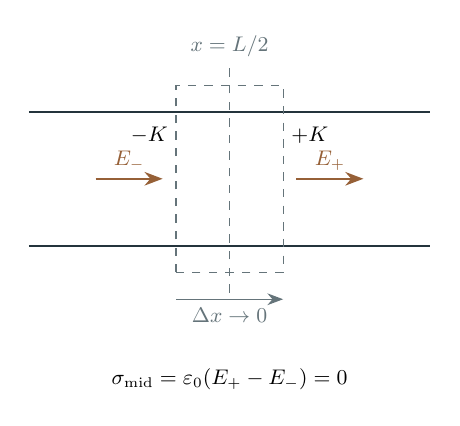
\begin{tikzpicture}[scale=.85,transform shape]

\draw[object] (-3,-1)--(3,-1);\draw[object] (-3,1)--(3,1);
\draw[guide] (0,-1.7)--(0,1.7) node[above] {$x=L/2$};
\draw[guide] (-.8,-1.4) rectangle (.8,1.4);
\draw[force] (-2,0)--(-1,0) node[midway,above] {$E_-$};
\draw[force] (1,0)--(2,0) node[midway,above] {$E_+$};
\draw[axis] (-.8,-1.8)--(.8,-1.8) node[midway,below] {$\Delta x\to0$};
\node at (0,-3) {$\sigma_{\rm mid}=\varepsilon_0(E_+-E_-)=0$};
\node[left] at (-.8,.65) {$-K$};\node[right] at (.8,.65) {$+K$};

\end{tikzpicture}
\figcaption{解图电试4.1B\quad 薄柱净通量由两侧场值差给出，有界体电荷在薄层内积分。}
\end{minipage}\end{center}
先让$h\to0$，体电荷在两侧有界，其总量的绝对值至多随$S_gh$趋零；截面若有有限面电荷，其总量则为$\sigma_{\rm mid}S_g$。高斯定律因此给
\[
\sigma_{\rm mid}=\varepsilon_0\bigl[E_x(L/2+0)-E_x(L/2-0)\bigr]
=\boxed{0}.
\]
两侧场值都趋于零，通量差随厚度趋零；两侧斜率分别给出有界的负、正体电荷。连续场的一阶分布导数只含上述有界体电荷，截面上没有额外的$\delta$项。

沿轴积分电场可得电势降，并把局部场与端电压联系起来。取$V(0)$为参考，$V(x)-V(0)=-\int_0^xE_x(\xi)\mathrm d\xi$。前半段直接积分正弦，
\[
V(x)=V(0)-\frac U4[1-\cos(2\pi x/L)],
\]
在中点先累积电势降$U/2$，再对后半段负正弦继续积分，得到
\[
V(x)=V(0)-\frac{3U}{4}-\frac U4\cos(2\pi x/L).
\]
\begin{center}\begin{minipage}{.98\linewidth}\centering
\begin{tikzpicture}[scale=.8,transform shape]
\draw[axis] (0,0)--(10.7,0) node[right] {$x/L$};
\draw[axis] (0,0)--(0,3.2) node[above] {$[V(0)-V(x)]/U$};\foreach \y/\lab in {0/0,1.4/0.5,2.8/1}{\draw[thin] (0,\y)--(-.08,\y) node[left] {$\lab$};}
\node[above] at (5,3.5) {电势降的累积量单调上升，中点为$1/2$};
\draw[traj] plot coordinates {(0.000000000,0.000000000) (0.083333333,0.000959326) (0.166666667,0.003834673) (0.250000000,0.008618162) (0.333333333,0.015296679) (0.416666667,0.023851922) (0.500000000,0.034260439) (0.583333333,0.046493701) (0.666666667,0.060518180) (0.750000000,0.076295433) (0.833333333,0.093782217) (0.916666667,0.112930602) (1.000000000,0.133688104) (1.083333333,0.155997827) (1.166666667,0.179798622) (1.250000000,0.205025253) (1.333333333,0.231608576) (1.416666667,0.259475726) (1.500000000,0.288550323) (1.583333333,0.318752675) (1.666666667,0.350000000) (1.750000000,0.382206650) (1.833333333,0.415284350) (1.916666667,0.449142435) (2.000000000,0.483688104) (2.083333333,0.518826668) (2.166666667,0.554461816) (2.250000000,0.590495874) (2.333333333,0.626830076) (2.416666667,0.663364831) (2.500000000,0.700000000) (2.583333333,0.736635169) (2.666666667,0.773169924) (2.750000000,0.809504126) (2.833333333,0.845538184) (2.916666667,0.881173332) (3.000000000,0.916311896) (3.083333333,0.950857565) (3.166666667,0.984715650) (3.250000000,1.017793350) (3.333333333,1.050000000) (3.416666667,1.081247325) (3.500000000,1.111449677) (3.583333333,1.140524274) (3.666666667,1.168391424) (3.750000000,1.194974747) (3.833333333,1.220201378) (3.916666667,1.244002173) (4.000000000,1.266311896) (4.083333333,1.287069398) (4.166666667,1.306217783) (4.250000000,1.323704567) (4.333333333,1.339481820) (4.416666667,1.353506299) (4.500000000,1.365739561) (4.583333333,1.376148078) (4.666666667,1.384703321) (4.750000000,1.391381838) (4.833333333,1.396165327) (4.916666667,1.399040674) (5.000000000,1.400000000) (5.083333333,1.400959326) (5.166666667,1.403834673) (5.250000000,1.408618162) (5.333333333,1.415296679) (5.416666667,1.423851922) (5.500000000,1.434260439) (5.583333333,1.446493701) (5.666666667,1.460518180) (5.750000000,1.476295433) (5.833333333,1.493782217) (5.916666667,1.512930602) (6.000000000,1.533688104) (6.083333333,1.555997827) (6.166666667,1.579798622) (6.250000000,1.605025253) (6.333333333,1.631608576) (6.416666667,1.659475726) (6.500000000,1.688550323) (6.583333333,1.718752675) (6.666666667,1.750000000) (6.750000000,1.782206650) (6.833333333,1.815284350) (6.916666667,1.849142435) (7.000000000,1.883688104) (7.083333333,1.918826668) (7.166666667,1.954461816) (7.250000000,1.990495874) (7.333333333,2.026830076) (7.416666667,2.063364831) (7.500000000,2.100000000) (7.583333333,2.136635169) (7.666666667,2.173169924) (7.750000000,2.209504126) (7.833333333,2.245538184) (7.916666667,2.281173332) (8.000000000,2.316311896) (8.083333333,2.350857565) (8.166666667,2.384715650) (8.250000000,2.417793350) (8.333333333,2.450000000) (8.416666667,2.481247325) (8.500000000,2.511449677) (8.583333333,2.540524274) (8.666666667,2.568391424) (8.750000000,2.594974747) (8.833333333,2.620201378) (8.916666667,2.644002173) (9.000000000,2.666311896) (9.083333333,2.687069398) (9.166666667,2.706217783) (9.250000000,2.723704567) (9.333333333,2.739481820) (9.416666667,2.753506299) (9.500000000,2.765739561) (9.583333333,2.776148078) (9.666666667,2.784703321) (9.750000000,2.791381838) (9.833333333,2.796165327) (9.916666667,2.799040674) (10.000000000,2.800000000)};
\node[below] at (0,-.12) {$0$};
\node[below] at (5,-.12) {$1/2$};
\node[below] at (10,-.12) {$1$};
\end{tikzpicture}
\figcaption{解图电试4.1C\quad 电势降的累积量单调上升，中点为$1/2$}
\end{minipage}\end{center}
解图电试4.1C画累计电势降$[V(0)-V(x)]/U$，中点为$1/2$，右端为1。电势连续下降，在场强为零的中点处斜率也为零。两段表达式在中点都给$V(0)-U/2$，右端给$V(L)=V(0)-U$。每半段的净体电荷为$\varepsilon_0S[E_x(x_{\rm right})-E_x(x_{\rm left})]=0$，与四段正负分布相容。两外端面的面电荷分别需要导体外侧的场值，端电压只给出内部场的积分。



\Needspace{13\baselineskip}

\pdfbookmark[2]{第 2 题 多端等效与无限内接三角形网络}{q2}

\section*{第 2 题\quad 多端等效与无限内接三角形网络}\label{q:2}


\begin{enumerate}
\item $N$端电阻网络可用外端两两之间的等效支路表示。说明这种表示中何时须允许开路支路，画出四端完全网络，以及一个由八个电阻组成、不能直接串并联约化的四端网络。
\item 等边三角形$ABC$的三边均被中点$P,Q,T$分为两段，每段电阻为$R$，三个中点之间也各接一个电阻$R$，其中$P$在$AB$、$Q$在$BC$、$T$在$CA$。求其对外端$A,B,C$的对称三角形等效网络。
\item 两个边长$a$的等边三角形$ABC$与$BCD$共边$BC$。左三角形中不断连接三边中点构成内接三角形，所有中点均电连接；右侧只增加$CD,DB$两段。各段为相同材料和粗细的金属丝，单位长度电阻$r$。求全网络$A,B$间等效电阻。
\end{enumerate}
无限网络按有限层截断、最内层不再加支路的极限定义。


\begin{center}\begin{minipage}{.98\linewidth}\centering
\begin{tikzpicture}[scale=.7,transform shape]

\coordinate (A) at (0,0);\coordinate (B) at (4,0);\coordinate (C) at (2,3.464);
\coordinate (P) at (2,0);\coordinate (Q) at (3,1.732);\coordinate (T) at (1,1.732);
\draw[object] (A)--(B)--(C)--cycle;\draw[object] (P)--(Q)--(T)--cycle;
\foreach \p/\pos in {A/below left,B/below right,C/above,P/below,Q/right,T/left}{\fill (\p) circle (1.6pt) node[\pos] {$\p$};}
\node at (2,-1) {每一小段均为$R$};\begin{scope}[xshift=7cm]
\coordinate (A) at (0,0);\coordinate (B) at (4,0);\coordinate (C) at (2,3.464);
\coordinate (D) at (6,3.464);
\draw[object] (A)--(B)--(C)--cycle;\draw[object] (C)--(D)--(B);
\foreach \k in {1,...,7}{
\coordinate (M) at ($(A)!.5!(B)$);\coordinate (N) at ($(B)!.5!(C)$);\coordinate (O) at ($(C)!.5!(A)$);
\draw[object] (M)--(N)--(O)--cycle;
\coordinate (A) at (M);\coordinate (B) at (N);\coordinate (C) at (O);}
\node[below left] at (0,0) {$A$};\node[below] at (4,0) {$B$};
\node[above] at (2,3.464) {$C$};\node[above right] at (6,3.464) {$D$};
\node[above] at (4,3.464) {$k=ar$};\node[right] at (5,1.732) {$k$};
\node at (3,-1) {左部无限内接，右部仅加两边};\end{scope}
\end{tikzpicture}
\figcaption{图电试4.2\quad 有限九电阻三角形与共边的无限三角形组合。}
\end{minipage}\end{center}

\Needspace{6\baselineskip}\subsection*{解答}


图电试4.2给出外端、内部结点及共边关系。多端等效要求对所有允许的外端电势给出相同的外端电流，仅匹配一次两端测量一般不足。

第（1）问，可把有限网络的结点导纳矩阵分成外端$b$与内部$i$两部分。内部无外注入电流，
\[
\begin{pmatrix}I_b\\0\end{pmatrix}
=\begin{pmatrix}Y_{bb}&Y_{bi}\\Y_{ib}&Y_{ii}\end{pmatrix}
\begin{pmatrix}V_b\\V_i\end{pmatrix},
\qquad
I_b=(Y_{bb}-Y_{bi}Y_{ii}^{-1}Y_{ib})V_b.
\]
内部方程先给$V_i=-Y_{ii}^{-1}Y_{ib}V_b$，代回外端方程即得上式。删去不连到外端的孤立部分后，任一保留的内部结点都有一条路通向外端。以解图电试4.2A右侧为例，固定四角外端的试探电势都为零，内部试探电势向量记为 $\boldsymbol v$。对每条边用端点电势差写耗散，得
\[
\boldsymbol v^{T}Y_{ii}\boldsymbol v
=\sum_{\{p,q\}} g_{pq}(v_p-v_q)^2 .
\]
右端每条边只计一次，$g_{pq}>0$。若和为零，各连通边的两端同势，沿路径一直到零势外端就知每个内部结点也为零。因此 $Y_{ii}$ 正定，可以逆求内部结点。约化矩阵的行和为零、非对角元非正，故可令外端$p,q$间支路电导
\[
g_{pq}=-(Y_{\rm eff})_{pq}\ge0.
\]
这些矩阵性质也可逐个消元说明。设一个内部结点与相邻结点分别以电导$g_1,\ldots,g_m$连接，记$G=\sum g_j$。内部无注入电流使其电势为$V_o=\sum g_jV_j/G$；代入相邻端电流，就在每对相邻点之间增加正电导$g_pg_q/G$。已有连接与新增电导相加，逐个消去全部内部结点后仍只有非负的两两电导，而且每个外端电流都由外端电势差相加给出。共同平移全部电势使电流保持相同，正是导纳矩阵行和为零的物理含义。外端彼此保持为独立接线点，内部结点则通过无注入电流条件消去，二者作用在这一步明确区分。

$g_{pq}>0$时电阻为$1/g_{pq}$，$g_{pq}=0$时该边开路。例子是三个结点全为外端的链$A-B-C$：它没有内部结点可消去，$AC$等效边电导为零，该端口对在完全图表示中保留为开路边。无限网络的这一表示需先确认截断网络的端口导纳极限存在。
\begin{center}\begin{minipage}{.98\linewidth}\centering
\begin{tikzpicture}[scale=.75,transform shape]

\draw[object] (0,0)--(4,0)--(4,3)--(0,3)--cycle;
\draw[object] (0,0)--(4,3);\draw[object] (0,3)--(4,0);
\draw[white,line width=4pt] (1.8,1.35)--(2.2,1.65);
\draw[object] (1.8,1.35)--(2.2,1.65);
\foreach \x/\y/\p in {0/0/A,4/0/B,4/3/C,0/3/D}{\fill (\x,\y) circle (2pt) node[above left] {$\p$};}
\node at (2,4) {六条边；交叉处不连接};
\begin{scope}[xshift=7cm]
\draw[object] (0,0)--(4,0)--(4,3)--(0,3)--cycle;
\foreach \x/\y/\p in {0/0/A,4/0/B,4/3/C,0/3/D}{
\draw[object] (\x,\y)--(2,1.5);
\fill (\x,\y) circle (2pt) node[above left] {$\p$};}
\fill (2,1.5) circle (2pt) node[right] {$O$};
\node at (2,4) {八电阻；中心为内部结点};
\end{scope}

\end{tikzpicture}
\figcaption{解图电试4.2A\quad 左图用跨线表示无结点交叉，右图中心明确电连接。}
\end{minipage}\end{center}
解图电试4.2A左侧四端完全网络共有$\binom42=6$条边，对角线交叉处不连接。右侧四边形四边及四条中心辐条共有八个电阻；四角均是外端，中心为内部结点，没有可直接串联合并的二度内部结点，也没有同端点并联边。

第（2）问，施加电流$I$从$A$流入、$B$流出，$C$不外接。取$V_B=0$、用$IR$作电势单位，记六点电势为$a,0,c,p,q,t$。结点方程为
\[
\begin{gathered}
2a-p-t=1,\quad 2c-q-t=0,\quad
4p-a-q-t=0,\\
4q-c-p-t=0,\quad
4t-a-c-p-q=0,\quad p+q=1.
\end{gathered}
\]
例如$P$点分别接$A,B,Q,T$四条$R$，所以$4p-a-q-t=0$；$A$点只有两条$R$向内连接，注入电流为$I$，给$2a-p-t=1$。最后一式为$B$的流出电流条件。解得
\[
(a,c,p,q,t)=\left(\frac{10}{9},\frac59,\frac59,\frac49,\frac23\right).
\]
可先用反对称电势得$c=p=a/2$，由$B$点条件得$q=1-a/2$，再由$P$点与$A$点方程消去$t$，得到$a=10/9$；其余电势随之确定。于是$R_{AB}=10R/9$。三外端完全对称，导纳约化后仍完全对称，三条等效边电阻必相等，设为$R_\Delta$。第三端开路时，
\[
R_{AB}=R_\Delta\parallel(2R_\Delta)=\frac23R_\Delta,
\qquad \boxed{R_\Delta=\frac53R}.
\]
这个对称性论证把一次两端计算提升为三端等效；这一步使用三外端的完整置换对称，一般三端网络需保留更多独立参数。
\begin{center}\begin{minipage}{.98\linewidth}\centering
\begin{tikzpicture}[scale=.8,transform shape]

\coordinate (A) at (0,0);\coordinate (B) at (4,0);\coordinate (C) at (2,3.464);
\coordinate (P) at (2,0);\coordinate (Q) at (3,1.732);\coordinate (T) at (1,1.732);
\draw[object] (A)--(B)--(C)--cycle;\draw[object] (P)--(Q)--(T)--cycle;
\foreach \p/\pos in {A/below left,B/below right,C/above,P/below,Q/right,T/left}{\fill (\p) circle (1.6pt) node[\pos] {$\p$};}

\node[align=left] at (7,1.7) {$V_A=+v,\ V_B=-v$\\$V_C=V_P=0$\\$V_T=w,\ V_Q=-w$};
\node at (2,4.6) {外半边$k/2$；内三角等效边$d=3X/4$};
\draw[motion] (-1,0)--(-.2,0) node[midway,above left] {$I$};

\end{tikzpicture}
\figcaption{解图电试4.2B\quad 反对称激励令两中性点为零电势，T点方程闭合自相似递推。}
\end{minipage}\end{center}
第（3）问，先只看左侧无限网络。记大边单边电阻$k=ar$，其$AB$两端电阻为$X$。解图电试4.2B中内接三角形尺度减半，所有电阻也减半，故其两端电阻为$X/2$，三端对称等效边为$d=3X/4$。

给$A,B$施加反对称电势$+v,-v$，由对称性$V_C=V_P=0$，令$V_T=w,V_Q=-w$。$T$点的两条外半边分别连$A,C$，两条内等效边分别连$P,Q$。前两条的电势差为$w-v,w$，后两条为$w,2w$，因此在$T$点列方程：
\[
\frac{w-v}{k/2}+\frac{w}{k/2}
+\frac{w}{d}+\frac{2w}{d}=0,
\qquad \frac wv=\frac{2d}{4d+3k}.
\]
外端$A$流入电流
\[
I=\frac{v}{k/2}+\frac{v-w}{k/2}
=\frac{4v-2w}{k}.
\]
这一步也可沿图D的分拆连接理解。外边中点$P$的电势为零，外侧$A\to P\to B$的流入、流出相等，内部$T\to P\to Q$也分别守恒，因此可把两个$P$分开。外边$AB$单独为$k$；上方路径中$T\to C\to Q$为$k$，它与小网两端的$X/2$并联，再与两侧各$k/2$串联，最后与直接边$k$并联。分拆只使用各子网的结点守恒，保持同一激励的电流。
\begin{center}\begin{minipage}{.98\linewidth}\centering
\begin{tikzpicture}[scale=.8,transform shape]
\coordinate (A) at (0,0);\coordinate (B) at (8,0);\coordinate (T) at (2,2);\coordinate (Q) at (6,2);\coordinate (C) at (4,4);\draw[thick] (A)--(T)--(C)--(Q)--(B)--cycle;\draw[line width=1.5pt,color=accent] (T)--(Q) node[midway,above] {$X/2$};\foreach \p in {A,B,T,Q,C}{\fill (\p) circle(.05) node[above left] {$\p$};}\node at (4,-.5) {$k$：外边$AB$单独保留};\node[left] at (1,1) {$k/2$};\node[right] at (7,1) {$k/2$};\node at (4,5) {$T-C-Q$串联为$k$，与$X/2$并联};
\end{tikzpicture}
\figcaption{解图电试4.2D\quad 将AB中点的内部、外部连接分拆，保留两侧中点之间的小网}
\end{minipage}\end{center}
所以
\[
X=\frac{2v}{I}
=\frac{k(4d+3k)}{6d+6k}
=\frac{k(k+X)}{2k+3X/2}.
\]
将分式两边乘分母，$X(2k+3X/2)=k(k+X)$，移项并乘2得到$3X^2+2kX-2k^2=0$。用求根式先得$X=k(-1\pm\sqrt7)/3$；正电阻对应其中正的根，取
\[
\boxed{X=\frac{\sqrt7-1}{3}k},\qquad
\boxed{R_\Delta^{(\infty)}=\frac32X=\frac{\sqrt7-1}{2}k}.
\]
题设的无限网络由有限截断定义，接着说明这一序列的极限。零层只有外三角形，$X_0=2k/3$；每增一内层，
\[
X_{n+1}=f(X_n),\quad
f(x)=\frac{k(k+x)}{2k+3x/2},\quad
0<f'(x)=\frac{k^2/2}{(2k+3x/2)^2}\le\frac18.
\]
由于$X_0$高于正固定点且$f$单调增加，有限层数值保持在固定点上方；增加内线又只增加导电通路，故逐层不增。此映射在正区间为压缩映射，有限截断唯一收敛到上述正根，误差至少按$1/8$逐次缩小。
\begin{center}\begin{minipage}{.98\linewidth}\centering
\begin{tikzpicture}[scale=.85,transform shape]

\draw[object] (0,0)--(4,0)--(2,3.464)--cycle;
\draw[object] (2,3.464)--(6,3.464)--(4,0);
\node[fill=white] at (2,0) {$d_\infty$};
\node[fill=white] at (.8,1.45) {$d_\infty$};
\node[fill=white] at (3.2,1.45) {$d_\infty$};
\node[fill=white] at (4,3.464) {$k$};
\node[fill=white] at (5,1.732) {$k$};
\node[below] at (0,0) {$A$};\node[below] at (4,0) {$B$};
\node[above] at (2,3.464) {$C$};\node[above] at (6,3.464) {$D$};
\node at (3,-1) {$d_\infty=\dfrac{\sqrt7-1}{2}k$，共边只计一次};

\end{tikzpicture}
\figcaption{解图电试4.2C\quad 左侧完整三端替换后，右侧CDB通路与等效BC边并联。}
\end{minipage}\end{center}
\begin{center}\begin{minipage}{.98\linewidth}\centering
\begin{tikzpicture}[scale=.8,transform shape]
\draw[axis] (0,0)--(10.7,0) node[right] {内接层数$n$};
\draw[axis] (0,0)--(0,3.2) node[above] {$R/k$};\foreach \y/\lab in {0/0,1.2/0.3,2.4/0.6}{\draw[thin] (0,\y)--(-.08,\y) node[left] {$\lab$};}
\node[above] at (5,3.5) {实线左网，虚线接入右侧两边；按同一有限层截断};
\draw[traj] plot coordinates {(0.000000000,2.666666667) (1.250000000,2.222222222) (2.500000000,2.196078431) (3.750000000,2.194444444) (5.000000000,2.194341943) (6.250000000,2.194335512) (7.500000000,2.194335108) (8.750000000,2.194335083) (10.000000000,2.194335082)};
\draw[dashed,thick,color=warm] plot coordinates {(0.000000000,2.500000000) (1.250000000,2.101449275) (2.500000000,2.077828054) (3.750000000,2.076351045) (5.000000000,2.076258388) (6.250000000,2.076252574) (7.500000000,2.076252210) (8.750000000,2.076252187) (10.000000000,2.076252185)};
\node[below] at (0,-.12) {$0$};
\node[below] at (5,-.12) {$4$};
\node[below] at (10,-.12) {$8$};
\end{tikzpicture}
\figcaption{解图电试4.2E\quad 实线左网，虚线接入右侧两边；按同一有限层截断}
\end{minipage}\end{center}
解图电试4.2E的两条曲线使用同样的最内层开端截断，左网先收敛，再把其完整三端关系接入右侧。解图电试4.2C将左部替换为三条$R_\Delta^{(\infty)}$，右侧仅保留$C-D-B$两段各$k$。共边$BC$已经包含在左部等效中，不再额外重复接一条$k$。

记$d_\infty=R_\Delta^{(\infty)}$，则$BC$间为$d_\infty\parallel2k$；$AB$间直接边与经$C$通路并联：
\[
\begin{aligned}
R_{AB}^{\rm all}
&=d_\infty\parallel[d_\infty+(d_\infty\parallel2k)]\\
&=\frac{d_\infty(d_\infty+4k)}{2(d_\infty+3k)}
=\boxed{\frac{5\sqrt7-7}{12}\,ar}.
\end{aligned}
\]
直接边为$d_\infty$，经$C$的另一通路为$d_\infty+(d_\infty\parallel2k)$；通路内部串联，通路之间并联，故有上式。代入$d_\infty/k=(\sqrt7-1)/2$再有理化，得到最后根式。它小于单独左网的$X$，符合新增被动导电支路不会增大端口电阻的判断。


\Needspace{13\baselineskip}

\pdfbookmark[2]{第 3 题 互补RL、RC支路的相量与初始储能}{q3}

\section*{第 3 题\quad 互补RL、RC支路的相量与初始储能}\label{q:3}


一电源给两条并联支路供电：一条为电阻$R$与电感$L$串联，另一条为电阻$R$与电容$C$串联。元件理想，电源内阻忽略。
\begin{enumerate}
\item 电动势$\mathcal E(t)=\mathcal E_0\sin^2\omega t$，且$\omega L=1/(\omega C)=R$。用相量图分析稳态两支路电流及总电流。
\item 电动势为具有傅里叶展开的任意周期函数。$L,C,R$满足什么关系时，稳态端口电流总为$i(t)=\mathcal E(t)/R$？用复导纳证明。
\item 在第（2）问所求匹配关系下，给出任意初始电感电流$i_L(0)$与电容电压$v_C(0)$时的端口电流，说明稳态结论的初始条件限制。
\end{enumerate}
电容电压取沿支路电流方向的电势降。


\begin{center}\begin{minipage}{.98\linewidth}\centering
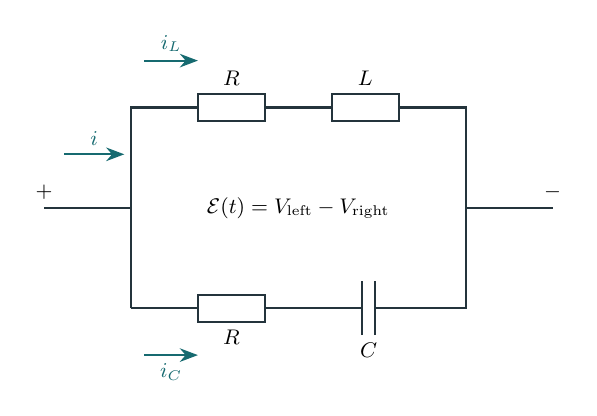
\begin{tikzpicture}[scale=.85,transform shape]

\draw[object] (0,0)--(0,3)--(1,3);
\draw[object] (1,2.8) rectangle (2,3.2);\node[above] at (1.5,3.2) {$R$};
\draw[object] (2,3)--(3,3);\draw[object] (3,2.8) rectangle (4,3.2);\node[above] at (3.5,3.2) {$L$};
\draw[object] (4,3)--(5,3)--(5,0)--(4,0);
\draw[object] (3.45,-.4)--(3.45,.4);\draw[object] (3.65,-.4)--(3.65,.4);
\draw[object] (4,0)--(3.65,0);\draw[object] (3.45,0)--(2,0);
\draw[object] (1,-.2) rectangle (2,.2);\node[below] at (1.5,-.2) {$R$};
\draw[object] (1,0)--(0,0);
\draw[object] (0,1.5)--(-1.3,1.5);\draw[object] (5,1.5)--(6.3,1.5);
\draw[motion] (-1,2.3)--(-.1,2.3) node[midway,above] {$i$};
\draw[motion] (.2,3.7)--(1,3.7) node[midway,above] {$i_L$};
\draw[motion] (.2,-.7)--(1,-.7) node[midway,below] {$i_C$};
\node[below] at (3.55,-.4) {$C$};
\node[above] at (-1.3,1.5) {$+$};\node[above] at (6.3,1.5) {$-$};
\node at (2.5,1.5) {$\mathcal E(t)=V_{\rm left}-V_{\rm right}$};

\end{tikzpicture}
\figcaption{图电试4.3\quad 两串联支路共用端电压，电流正方向均从左到右。}
\end{minipage}\end{center}

\Needspace{6\baselineskip}\subsection*{解答}


图电试4.3中两支路共用同一端电压，总电流是支路电流的代数和。先展开电源：
\[
\mathcal E(t)=\frac{\mathcal E_0}{2}
-\frac{\mathcal E_0}{2}\cos2\omega t.
\]
输入分成直流和$2\omega$交流，后者的两支路电抗分别由$2\omega L$与$1/(2\omega C)$确定。

直流稳态时电感短接、电容开路，所以
\[
i_{L,{\rm dc}}=\frac{\mathcal E_0}{2R},\qquad
i_{C,{\rm dc}}=0.
\]
对交流分量记幅值$E_a=\mathcal E_0/2$、角频率$\Omega=2\omega$，则
\[
X_L=\Omega L=2R,\qquad X_C=\frac1{\Omega C}=\frac R2.
\]
\begin{center}\begin{minipage}{.98\linewidth}\centering
\begin{tikzpicture}[scale=.75,transform shape]

\node at (1.8,3.7) {支路电压三角形};
\draw[axis] (0,0)--(3.5,0) node[right] {$\widetilde E_a$};
\draw[motion] (0,0)--(.6,-1.2) node[midway,left] {$RI_{La}$};
\draw[force] (.6,-1.2)--(3,0) node[midway,below] {$2RI_{La}$};
\draw[motion] (0,0)--(2.4,1.2) node[midway,above left] {$RI_{Ca}$};
\draw[force] (2.4,1.2)--(3,0) node[midway,right] {$RI_{Ca}/2$};
\node at (1.8,-2.4) {$\phi_L+\phi_C=90^\circ$};
\begin{scope}[xshift=6cm]
\node at (1.8,3.7) {支路电流相加};
\draw[axis] (0,0)--(4.4,0) node[right] {同相};
\draw[axis] (0,-2.1)--(0,2.1);
\draw[motion] (0,0)--(.7,-1.4) node[below right] {$\widetilde I_{La}$};
\draw[motion] (0,0)--(2.8,1.4) node[above] {$\widetilde I_{Ca}$};
\draw[guide] (.7,-1.4)--(3.5,0)--(2.8,1.4);
\draw[force] (0,.08)--(3.5,.08) node[midway,above] {$\widetilde I_a=\widetilde E_a/R$};
\end{scope}

\end{tikzpicture}
\figcaption{解图电试4.3A\quad 先以交流电压为参考作图，再恢复输入负余弦的相位。}
\end{minipage}\end{center}
\begin{center}\begin{minipage}{.98\linewidth}\centering
\begin{tikzpicture}[scale=.8,transform shape]
\draw[axis] (0,0)--(2.8,0) node[right] {$I_L$};\draw[motion] (0,0)--(1,0) node[midway,below] {$I_LR$};\draw[motion] (1,0)--(1,2) node[midway,right] {$2I_LR$};\draw[force] (0,0)--(1,2) node[above] {$E_a$};\draw (0.5,0) arc(0:63.434949:.5);\node at (.8,.4) {$\phi_L$};\begin{scope}[xshift=6cm]\draw[axis] (0,0)--(3,0) node[right] {$I_C$};\draw[motion] (0,0)--(2,0) node[midway,above] {$I_CR$};\draw[motion] (2,0)--(2,-1) node[midway,right] {$I_CR/2$};\draw[force] (0,0)--(2,-1) node[right] {$E_a$};\draw (.6,0) arc(0:-26.565051:.6);\node at (1,-.5) {$\phi_C$};\end{scope}\node at (3,3) {两幅图各以支路电流为水平参考；电压横纵同尺度};
\end{tikzpicture}
\figcaption{解图电试4.3D\quad 两支路串联电压直角三角形决定电流相对端电压的相位}
\end{minipage}\end{center}
解图电试4.3D中两幅支路电压图各自以电流为参考：$RL$的水平电阻电压为$I_LR$，竖直向上电感电压为$2I_LR$；$RC$的水平电阻电压为$I_CR$，竖直向下电容电压为$I_CR/2$。电源电压都是同一条支路两电压的矢量和，故分别形成直角三角形。把每幅图旋到电源电压水平的共同参考后，再相加两电流。

解图电试4.3A以该交流电压相量$\widetilde E_a$为水平参考；$RL$支路的电阻电压与电流同相、电感电压超前电流$90^\circ$，两者直角相加。$RC$支路的电容电压落后电流$90^\circ$。据两个电压三角形，
\[
I_{La}=\frac{E_a}{\sqrt{R^2+(2R)^2}}
=\frac{E_a}{\sqrt5R},\qquad
I_{Ca}=\frac{E_a}{\sqrt{R^2+(R/2)^2}}
=\frac{2E_a}{\sqrt5R},
\]
\[
\tan\phi_L=2,\qquad \tan\phi_C=\frac12,\qquad
\phi_L+\phi_C=\frac\pi2.
\]
两支路电流相量互相垂直。电流的同相、正交分量分别为
\[
\begin{aligned}
I_{La}\cos\phi_L&=\frac{E_a}{5R},&
I_{La}\sin\phi_L&=\frac{2E_a}{5R},\\
I_{Ca}\cos\phi_C&=\frac{4E_a}{5R},&
I_{Ca}\sin\phi_C&=\frac{2E_a}{5R}.
\end{aligned}
\]
两电流与参考电压的夹角分别在下方$\phi_L$、上方$\phi_C$，所以第一支路的正交分量为负、第二支路为正；它们大小均为$2E_a/(5R)$。水平分量$E_a/(5R)+4E_a/(5R)=E_a/R$。也可由两电流互相垂直，以勾股关系得到合电流幅值$\sqrt{I_{La}^2+I_{Ca}^2}=E_a/R$，其方向由正交分量的相消确定。正交分量抵消，同相分量相加得$E_a/R$。代回输入交流项的负号，完整支路电流可写为
\[
\begin{aligned}
i_L(t)&=\frac{\mathcal E_0}{2R}
-\frac{\mathcal E_0}{10R}\cos2\omega t
-\frac{\mathcal E_0}{5R}\sin2\omega t,\\
i_C(t)&=-\frac{2\mathcal E_0}{5R}\cos2\omega t
+\frac{\mathcal E_0}{5R}\sin2\omega t.
\end{aligned}
\]
因此
\[
\boxed{i(t)=\frac{\mathcal E_0}{2R}(1-\cos2\omega t)
=\frac{\mathcal E_0}{R}\sin^2\omega t}.
\]
电容支路电流可以为负，总电流却始终非负。相量图只处理单一频率的交流分量，直流须另外叠加。

\begin{center}\begin{minipage}{.98\linewidth}\centering
\begin{tikzpicture}[scale=.8,transform shape]
\draw[axis] (0,0)--(10.7,0) node[right] {$\omega t$};
\draw[axis] (0,0)--(0,3.2) node[above] {$iR/\mathcal E_0$};\foreach \y/\lab in {0/-0.5,1.8/0.5,2.7/1}{\draw[thin] (0,\y)--(-.08,\y) node[left] {$\lab$};}
\node[above] at (5,3.5) {实线RL、虚线RC、细线端口；水平点线为零电流};
\draw[traj] plot coordinates {(0.000000000,1.620000000) (0.062500000,1.592309605) (0.125000000,1.565899691) (0.187500000,1.540933083) (0.250000000,1.517563709) (0.312500000,1.495935648) (0.375000000,1.476182246) (0.437500000,1.458425287) (0.500000000,1.442774250) (0.562500000,1.429325629) (0.625000000,1.418162338) (0.687500000,1.409353204) (0.750000000,1.402952537) (0.812500000,1.398999799) (0.875000000,1.397519361) (0.937500000,1.398520350) (1.000000000,1.401996595) (1.062500000,1.407926663) (1.125000000,1.416273994) (1.187500000,1.426987123) (1.250000000,1.440000000) (1.312500000,1.455232397) (1.375000000,1.472590401) (1.437500000,1.491966994) (1.500000000,1.513242713) (1.562500000,1.536286386) (1.625000000,1.560955941) (1.687500000,1.587099282) (1.750000000,1.614555227) (1.812500000,1.643154501) (1.875000000,1.672720779) (1.937500000,1.703071776) (2.000000000,1.734020368) (2.062500000,1.765375746) (2.125000000,1.796944594) (2.187500000,1.828532280) (2.250000000,1.859944055) (2.312500000,1.890986255) (2.375000000,1.921467494) (2.437500000,1.951199846) (2.500000000,1.980000000) (2.562500000,2.007690395) (2.625000000,2.034100309) (2.687500000,2.059066917) (2.750000000,2.082436291) (2.812500000,2.104064352) (2.875000000,2.123817754) (2.937500000,2.141574713) (3.000000000,2.157225750) (3.062500000,2.170674371) (3.125000000,2.181837662) (3.187500000,2.190646796) (3.250000000,2.197047463) (3.312500000,2.201000201) (3.375000000,2.202480639) (3.437500000,2.201479650) (3.500000000,2.198003405) (3.562500000,2.192073337) (3.625000000,2.183726006) (3.687500000,2.173012877) (3.750000000,2.160000000) (3.812500000,2.144767603) (3.875000000,2.127409599) (3.937500000,2.108033006) (4.000000000,2.086757287) (4.062500000,2.063713614) (4.125000000,2.039044059) (4.187500000,2.012900718) (4.250000000,1.985444773) (4.312500000,1.956845499) (4.375000000,1.927279221) (4.437500000,1.896928224) (4.500000000,1.865979632) (4.562500000,1.834624254) (4.625000000,1.803055406) (4.687500000,1.771467720) (4.750000000,1.740055945) (4.812500000,1.709013745) (4.875000000,1.678532506) (4.937500000,1.648800154) (5.000000000,1.620000000) (5.062500000,1.592309605) (5.125000000,1.565899691) (5.187500000,1.540933083) (5.250000000,1.517563709) (5.312500000,1.495935648) (5.375000000,1.476182246) (5.437500000,1.458425287) (5.500000000,1.442774250) (5.562500000,1.429325629) (5.625000000,1.418162338) (5.687500000,1.409353204) (5.750000000,1.402952537) (5.812500000,1.398999799) (5.875000000,1.397519361) (5.937500000,1.398520350) (6.000000000,1.401996595) (6.062500000,1.407926663) (6.125000000,1.416273994) (6.187500000,1.426987123) (6.250000000,1.440000000) (6.312500000,1.455232397) (6.375000000,1.472590401) (6.437500000,1.491966994) (6.500000000,1.513242713) (6.562500000,1.536286386) (6.625000000,1.560955941) (6.687500000,1.587099282) (6.750000000,1.614555227) (6.812500000,1.643154501) (6.875000000,1.672720779) (6.937500000,1.703071776) (7.000000000,1.734020368) (7.062500000,1.765375746) (7.125000000,1.796944594) (7.187500000,1.828532280) (7.250000000,1.859944055) (7.312500000,1.890986255) (7.375000000,1.921467494) (7.437500000,1.951199846) (7.500000000,1.980000000) (7.562500000,2.007690395) (7.625000000,2.034100309) (7.687500000,2.059066917) (7.750000000,2.082436291) (7.812500000,2.104064352) (7.875000000,2.123817754) (7.937500000,2.141574713) (8.000000000,2.157225750) (8.062500000,2.170674371) (8.125000000,2.181837662) (8.187500000,2.190646796) (8.250000000,2.197047463) (8.312500000,2.201000201) (8.375000000,2.202480639) (8.437500000,2.201479650) (8.500000000,2.198003405) (8.562500000,2.192073337) (8.625000000,2.183726006) (8.687500000,2.173012877) (8.750000000,2.160000000) (8.812500000,2.144767603) (8.875000000,2.127409599) (8.937500000,2.108033006) (9.000000000,2.086757287) (9.062500000,2.063713614) (9.125000000,2.039044059) (9.187500000,2.012900718) (9.250000000,1.985444773) (9.312500000,1.956845499) (9.375000000,1.927279221) (9.437500000,1.896928224) (9.500000000,1.865979632) (9.562500000,1.834624254) (9.625000000,1.803055406) (9.687500000,1.771467720) (9.750000000,1.740055945) (9.812500000,1.709013745) (9.875000000,1.678532506) (9.937500000,1.648800154) (10.000000000,1.620000000)};
\draw[dashed,thick,color=warm] plot coordinates {(0.000000000,0.180000000) (0.062500000,0.210464794) (0.125000000,0.245180802) (0.187500000,0.283933988) (0.250000000,0.326485426) (0.312500000,0.372572772) (0.375000000,0.421911882) (0.437500000,0.474198565) (0.500000000,0.529110455) (0.562500000,0.586309002) (0.625000000,0.645441559) (0.687500000,0.706143553) (0.750000000,0.768040736) (0.812500000,0.830751493) (0.875000000,0.893889189) (0.937500000,0.957064560) (1.000000000,1.019888110) (1.062500000,1.081972509) (1.125000000,1.142934988) (1.187500000,1.202399691) (1.250000000,1.260000000) (1.312500000,1.315380789) (1.375000000,1.368200617) (1.437500000,1.418133833) (1.500000000,1.464872582) (1.562500000,1.508128703) (1.625000000,1.547635509) (1.687500000,1.583149426) (1.750000000,1.614451500) (1.812500000,1.641348742) (1.875000000,1.663675324) (1.937500000,1.681293593) (2.000000000,1.694094927) (2.062500000,1.702000402) (2.125000000,1.704961277) (2.187500000,1.702959299) (2.250000000,1.696006810) (2.312500000,1.684146674) (2.375000000,1.667452013) (2.437500000,1.646025755) (2.500000000,1.620000000) (2.562500000,1.589535206) (2.625000000,1.554819198) (2.687500000,1.516066012) (2.750000000,1.473514574) (2.812500000,1.427427228) (2.875000000,1.378088118) (2.937500000,1.325801435) (3.000000000,1.270889545) (3.062500000,1.213690998) (3.125000000,1.154558441) (3.187500000,1.093856447) (3.250000000,1.031959264) (3.312500000,0.969248507) (3.375000000,0.906110811) (3.437500000,0.842935440) (3.500000000,0.780111890) (3.562500000,0.718027491) (3.625000000,0.657065012) (3.687500000,0.597600309) (3.750000000,0.540000000) (3.812500000,0.484619211) (3.875000000,0.431799383) (3.937500000,0.381866167) (4.000000000,0.335127418) (4.062500000,0.291871297) (4.125000000,0.252364491) (4.187500000,0.216850574) (4.250000000,0.185548500) (4.312500000,0.158651258) (4.375000000,0.136324676) (4.437500000,0.118706407) (4.500000000,0.105905073) (4.562500000,0.097999598) (4.625000000,0.095038723) (4.687500000,0.097040701) (4.750000000,0.103993190) (4.812500000,0.115853326) (4.875000000,0.132547987) (4.937500000,0.153974245) (5.000000000,0.180000000) (5.062500000,0.210464794) (5.125000000,0.245180802) (5.187500000,0.283933988) (5.250000000,0.326485426) (5.312500000,0.372572772) (5.375000000,0.421911882) (5.437500000,0.474198565) (5.500000000,0.529110455) (5.562500000,0.586309002) (5.625000000,0.645441559) (5.687500000,0.706143553) (5.750000000,0.768040736) (5.812500000,0.830751493) (5.875000000,0.893889189) (5.937500000,0.957064560) (6.000000000,1.019888110) (6.062500000,1.081972509) (6.125000000,1.142934988) (6.187500000,1.202399691) (6.250000000,1.260000000) (6.312500000,1.315380789) (6.375000000,1.368200617) (6.437500000,1.418133833) (6.500000000,1.464872582) (6.562500000,1.508128703) (6.625000000,1.547635509) (6.687500000,1.583149426) (6.750000000,1.614451500) (6.812500000,1.641348742) (6.875000000,1.663675324) (6.937500000,1.681293593) (7.000000000,1.694094927) (7.062500000,1.702000402) (7.125000000,1.704961277) (7.187500000,1.702959299) (7.250000000,1.696006810) (7.312500000,1.684146674) (7.375000000,1.667452013) (7.437500000,1.646025755) (7.500000000,1.620000000) (7.562500000,1.589535206) (7.625000000,1.554819198) (7.687500000,1.516066012) (7.750000000,1.473514574) (7.812500000,1.427427228) (7.875000000,1.378088118) (7.937500000,1.325801435) (8.000000000,1.270889545) (8.062500000,1.213690998) (8.125000000,1.154558441) (8.187500000,1.093856447) (8.250000000,1.031959264) (8.312500000,0.969248507) (8.375000000,0.906110811) (8.437500000,0.842935440) (8.500000000,0.780111890) (8.562500000,0.718027491) (8.625000000,0.657065012) (8.687500000,0.597600309) (8.750000000,0.540000000) (8.812500000,0.484619211) (8.875000000,0.431799383) (8.937500000,0.381866167) (9.000000000,0.335127418) (9.062500000,0.291871297) (9.125000000,0.252364491) (9.187500000,0.216850574) (9.250000000,0.185548500) (9.312500000,0.158651258) (9.375000000,0.136324676) (9.437500000,0.118706407) (9.500000000,0.105905073) (9.562500000,0.097999598) (9.625000000,0.095038723) (9.687500000,0.097040701) (9.750000000,0.103993190) (9.812500000,0.115853326) (9.875000000,0.132547987) (9.937500000,0.153974245) (10.000000000,0.180000000)};
\draw[thin,color=black] plot coordinates {(0.000000000,0.900000000) (0.062500000,0.902774400) (0.125000000,0.911080493) (0.187500000,0.924867072) (0.250000000,0.944049135) (0.312500000,0.968508421) (0.375000000,0.998094128) (0.437500000,1.032623852) (0.500000000,1.071884705) (0.562500000,1.115634631) (0.625000000,1.163603897) (0.687500000,1.215496757) (0.750000000,1.270993273) (0.812500000,1.329751292) (0.875000000,1.391408550) (0.937500000,1.455584911) (1.000000000,1.521884705) (1.062500000,1.589899173) (1.125000000,1.659208981) (1.187500000,1.729386814) (1.250000000,1.800000000) (1.312500000,1.870613186) (1.375000000,1.940791019) (1.437500000,2.010100827) (1.500000000,2.078115295) (1.562500000,2.144415089) (1.625000000,2.208591450) (1.687500000,2.270248708) (1.750000000,2.329006727) (1.812500000,2.384503243) (1.875000000,2.436396103) (1.937500000,2.484365369) (2.000000000,2.528115295) (2.062500000,2.567376148) (2.125000000,2.601905872) (2.187500000,2.631491579) (2.250000000,2.655950865) (2.312500000,2.675132928) (2.375000000,2.688919507) (2.437500000,2.697225600) (2.500000000,2.700000000) (2.562500000,2.697225600) (2.625000000,2.688919507) (2.687500000,2.675132928) (2.750000000,2.655950865) (2.812500000,2.631491579) (2.875000000,2.601905872) (2.937500000,2.567376148) (3.000000000,2.528115295) (3.062500000,2.484365369) (3.125000000,2.436396103) (3.187500000,2.384503243) (3.250000000,2.329006727) (3.312500000,2.270248708) (3.375000000,2.208591450) (3.437500000,2.144415089) (3.500000000,2.078115295) (3.562500000,2.010100827) (3.625000000,1.940791019) (3.687500000,1.870613186) (3.750000000,1.800000000) (3.812500000,1.729386814) (3.875000000,1.659208981) (3.937500000,1.589899173) (4.000000000,1.521884705) (4.062500000,1.455584911) (4.125000000,1.391408550) (4.187500000,1.329751292) (4.250000000,1.270993273) (4.312500000,1.215496757) (4.375000000,1.163603897) (4.437500000,1.115634631) (4.500000000,1.071884705) (4.562500000,1.032623852) (4.625000000,0.998094128) (4.687500000,0.968508421) (4.750000000,0.944049135) (4.812500000,0.924867072) (4.875000000,0.911080493) (4.937500000,0.902774400) (5.000000000,0.900000000) (5.062500000,0.902774400) (5.125000000,0.911080493) (5.187500000,0.924867072) (5.250000000,0.944049135) (5.312500000,0.968508421) (5.375000000,0.998094128) (5.437500000,1.032623852) (5.500000000,1.071884705) (5.562500000,1.115634631) (5.625000000,1.163603897) (5.687500000,1.215496757) (5.750000000,1.270993273) (5.812500000,1.329751292) (5.875000000,1.391408550) (5.937500000,1.455584911) (6.000000000,1.521884705) (6.062500000,1.589899173) (6.125000000,1.659208981) (6.187500000,1.729386814) (6.250000000,1.800000000) (6.312500000,1.870613186) (6.375000000,1.940791019) (6.437500000,2.010100827) (6.500000000,2.078115295) (6.562500000,2.144415089) (6.625000000,2.208591450) (6.687500000,2.270248708) (6.750000000,2.329006727) (6.812500000,2.384503243) (6.875000000,2.436396103) (6.937500000,2.484365369) (7.000000000,2.528115295) (7.062500000,2.567376148) (7.125000000,2.601905872) (7.187500000,2.631491579) (7.250000000,2.655950865) (7.312500000,2.675132928) (7.375000000,2.688919507) (7.437500000,2.697225600) (7.500000000,2.700000000) (7.562500000,2.697225600) (7.625000000,2.688919507) (7.687500000,2.675132928) (7.750000000,2.655950865) (7.812500000,2.631491579) (7.875000000,2.601905872) (7.937500000,2.567376148) (8.000000000,2.528115295) (8.062500000,2.484365369) (8.125000000,2.436396103) (8.187500000,2.384503243) (8.250000000,2.329006727) (8.312500000,2.270248708) (8.375000000,2.208591450) (8.437500000,2.144415089) (8.500000000,2.078115295) (8.562500000,2.010100827) (8.625000000,1.940791019) (8.687500000,1.870613186) (8.750000000,1.800000000) (8.812500000,1.729386814) (8.875000000,1.659208981) (8.937500000,1.589899173) (9.000000000,1.521884705) (9.062500000,1.455584911) (9.125000000,1.391408550) (9.187500000,1.329751292) (9.250000000,1.270993273) (9.312500000,1.215496757) (9.375000000,1.163603897) (9.437500000,1.115634631) (9.500000000,1.071884705) (9.562500000,1.032623852) (9.625000000,0.998094128) (9.687500000,0.968508421) (9.750000000,0.944049135) (9.812500000,0.924867072) (9.875000000,0.911080493) (9.937500000,0.902774400) (10.000000000,0.900000000)};
\node[below] at (0,-.12) {$0$};
\node[below] at (5,-.12) {$\pi$};
\node[below] at (10,-.12) {$2\pi$};
\draw[dotted] (0,.9)--(10,.9);\node[left] at (0,.9) {$0$};
\end{tikzpicture}
\figcaption{解图电试4.3C\quad 实线RL、虚线RC、细线端口；水平点线为零电流}
\end{minipage}\end{center}
解图电试4.3C在$t=0$给$i_L=2\mathcal E_0/(5R)$、$i_C=-2\mathcal E_0/(5R)$，两者相加为零。图中已经是周期稳态，电感、电容保存的瞬时状态使内部电流可在端口过零时继续存在。两支路的正弦正交项相反，余弦项与直流相加后形成非负的端口平方正弦。

第（2）问，任一非零角频率$\Omega$的输入电压相量记为$\widetilde E$。两支路导纳相加：
\[
Y(\Omega)=\frac1{R+\mathrm j\Omega L}
+\frac{\mathrm j\Omega C}{1+\mathrm j\Omega RC}.
\]
当
\[
\boxed{L=R^2C}
\]
时，时间常数满足$L/R=RC$。第一导纳的分母可写成$R(1+j\Omega RC)$，第二导纳已有同一因子，因此两个分母相同，故
\[
Y(\Omega)=\frac{1/R+\mathrm j\Omega C}
{1+\mathrm j\Omega RC}=\boxed{\frac1R}.
\]
通分时先把$1/R$写在同一分母下，分子中的常量和$\Omega^2LC$项逐项抵消，只剩与$R^2C-L$成正比的一阶虚数项。反过来，令$Y-1/R=0$，通分得
\[
Y-\frac1R=
\frac{\mathrm j\Omega(R^2C-L)}
{R(R+\mathrm j\Omega L)(1+\mathrm j\Omega RC)}.
\]
要在任一非零频率恒等于零，即得到同一匹配条件。直流导纳也为$1/R$，于是对
\[
\mathcal E(t)=E_{\rm dc}
+\sum_{n\ge1}E_n\cos(\Omega_nt+\psi_n)
\]
逐频率相加，稳态总电流恰为$\mathcal E(t)/R$。零初态时，相同的拉普拉斯导纳恒等式适用于一般分段连续输入，涵盖非周期驱动。
\begin{center}\begin{minipage}{.98\linewidth}\centering
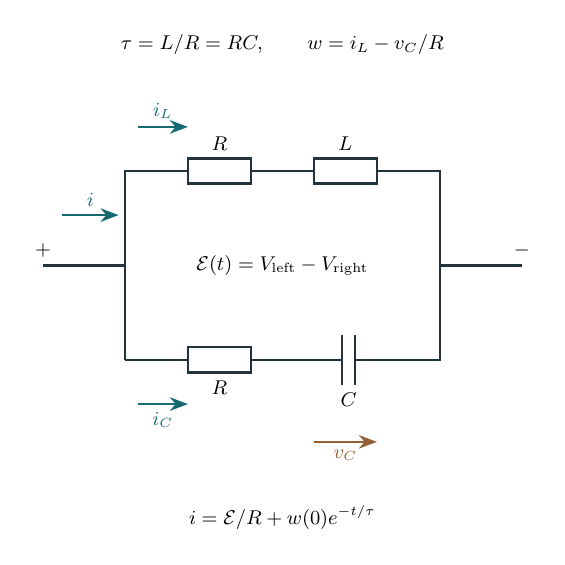
\begin{tikzpicture}[scale=.8,transform shape]

\draw[object] (0,0)--(0,3)--(1,3);
\draw[object] (1,2.8) rectangle (2,3.2);\node[above] at (1.5,3.2) {$R$};
\draw[object] (2,3)--(3,3);\draw[object] (3,2.8) rectangle (4,3.2);\node[above] at (3.5,3.2) {$L$};
\draw[object] (4,3)--(5,3)--(5,0)--(4,0);
\draw[object] (3.45,-.4)--(3.45,.4);\draw[object] (3.65,-.4)--(3.65,.4);
\draw[object] (4,0)--(3.65,0);\draw[object] (3.45,0)--(2,0);
\draw[object] (1,-.2) rectangle (2,.2);\node[below] at (1.5,-.2) {$R$};
\draw[object] (1,0)--(0,0);
\draw[object] (0,1.5)--(-1.3,1.5);\draw[object] (5,1.5)--(6.3,1.5);
\draw[motion] (-1,2.3)--(-.1,2.3) node[midway,above] {$i$};
\draw[motion] (.2,3.7)--(1,3.7) node[midway,above] {$i_L$};
\draw[motion] (.2,-.7)--(1,-.7) node[midway,below] {$i_C$};
\node[below] at (3.55,-.4) {$C$};
\node[above] at (-1.3,1.5) {$+$};\node[above] at (6.3,1.5) {$-$};
\node at (2.5,1.5) {$\mathcal E(t)=V_{\rm left}-V_{\rm right}$};

\draw[force] (3,-1.3)--(4,-1.3) node[midway,below] {$v_C$};
\node at (2.5,5) {$\tau=L/R=RC,\qquad w=i_L-v_C/R$};
\node at (2.5,-2.5) {$i=\mathcal E/R+w(0)e^{-t/\tau}$};

\end{tikzpicture}
\figcaption{解图电试4.3B\quad 保留初始电感电流和电容电压，端口额外响应由状态差决定。}
\end{minipage}\end{center}
第（3）问中，解图电试4.3B保留了电感、电容中的初始储能。支路方程为
\[
L\dot i_L+Ri_L=\mathcal E,\qquad
RC\dot v_C+v_C=\mathcal E,\qquad
i_C=\frac{\mathcal E-v_C}{R}.
\]
对电感方程除以$L$，对电容方程除以$R^2C$，匹配后两式的驱动项都是$\mathcal E/(R^2C)$，状态项系数都是$1/(RC)$。在$L=R^2C$下令$w=i_L-v_C/R$，相减可得
\[
\dot w=-\frac{w}{RC},\qquad
w(t)=\left[i_L(0)-\frac{v_C(0)}R\right]e^{-t/(RC)}.
\]
因此一般端口响应为
\[
\boxed{i(t)=\frac{\mathcal E(t)}R+
\left[i_L(0)-\frac{v_C(0)}R\right]e^{-t/(RC)}}.
\]
零状态、匹配初态$i_L(0)=v_C(0)/R$，以及暂态衰减后的稳态，都给端口纯电阻关系。即使初始能量非零，只要$w(0)=0$，这一自然响应也可在端口完全抵消；内部电流、电压及耗散仍实际存在。
这里总电流的恒等分解是$i=i_L+(\mathcal E-v_C)/R=\mathcal E/R+w$。状态差的一阶齐次方程中驱动完全相消，积分得到指数项，说明它的系数只由两个初值确定。电容电压取沿支路电流方向的电势降，所以它在$w$中带负号；电感电流取电源流入支路的方向，在$w$中带正号。匹配的内部状态仍有储能，并通过两电阻逐渐耗散。



\Needspace{13\baselineskip}

\pdfbookmark[2]{第 4 题 双行CLC网络的复阻抗和功率因数}{q4}

\section*{第 4 题\quad 双行CLC网络的复阻抗和功率因数}\label{q:4}


如图，两条水平支路各依次由电容$C$、电感$L$、电容$C$连接而成；四列上下对应结点之间均接电阻$R$。以左下结点$A$和右上结点$B$为端口。
\begin{enumerate}
\item 求角频率$\omega$下的端口复阻抗$Z$。
\item 当$\omega L=1/(\omega C)=R$时，求$|Z|$和功率因数，说明电流相位。
\end{enumerate}
所有同名元件参数相同；用电流从$A$流入、从$B$流出的方向定义端口电压。


\begin{center}\begin{minipage}{.98\linewidth}\centering
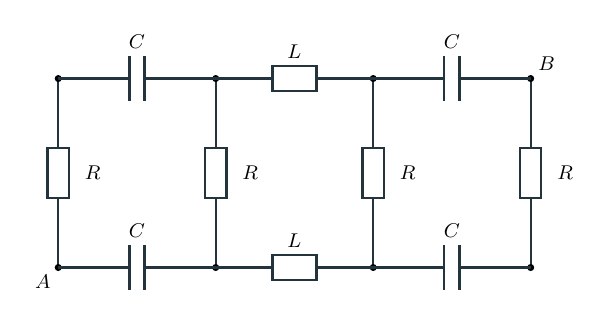
\begin{tikzpicture}[scale=.8,transform shape]

\foreach \x in {0,2.5,5,7.5}{
\draw[object] (\x,0)--(\x,1.1);
\draw[object] ({\x-.17},1.1) rectangle ({\x+.17},1.9);
\draw[object] (\x,1.9)--(\x,3);
\node[right] at ({\x+.3},1.5) {$R$};
\fill (\x,0) circle (1.6pt);\fill (\x,3) circle (1.6pt);}
\foreach \y in {0,3}{
\foreach \a/\b in {0/2.5,5/7.5}{
\pgfmathsetmacro{\m}{(\a+\b)/2}
\draw[object] (\a,\y)--({\m-.12},\y);
\draw[object] ({\m+.12},\y)--(\b,\y);
\draw[object] ({\m-.12},{\y-.35})--({\m-.12},{\y+.35});
\draw[object] ({\m+.12},{\y-.35})--({\m+.12},{\y+.35});
\node[above] at (\m,{\y+.35}) {$C$};}
\draw[object] (2.5,\y)--(3.4,\y);
\draw[object] (3.4,{\y-.2}) rectangle (4.1,{\y+.2});
\draw[object] (4.1,\y)--(5,\y);\node[above] at (3.75,{\y+.2}) {$L$};}
\node[below left] at (0,0) {$A$};\node[above right] at (7.5,3) {$B$};

\end{tikzpicture}
\figcaption{图电试4.4\quad 上下均为CLC，四列竖直电阻相同；端口在对角两端。}
\end{minipage}\end{center}

\Needspace{6\baselineskip}\subsection*{解答}


图电试4.4关于中心旋转$180^\circ$后互换端口。将端口电势取为$+V/2,-V/2$，由线性与唯一性，对应结点电势互为相反数；对应支路的代数电流据此配对。
\begin{center}\begin{minipage}{.98\linewidth}\centering
\begin{tikzpicture}[scale=.8,transform shape]

\foreach \x in {0,2.5,5,7.5}{
\draw[object] (\x,0)--(\x,1.1);
\draw[object] ({\x-.17},1.1) rectangle ({\x+.17},1.9);
\draw[object] (\x,1.9)--(\x,3);
\node[right] at ({\x+.3},1.5) {$R$};
\fill (\x,0) circle (1.6pt);\fill (\x,3) circle (1.6pt);}
\foreach \y in {0,3}{
\foreach \a/\b in {0/2.5,5/7.5}{
\pgfmathsetmacro{\m}{(\a+\b)/2}
\draw[object] (\a,\y)--({\m-.12},\y);
\draw[object] ({\m+.12},\y)--(\b,\y);
\draw[object] ({\m-.12},{\y-.35})--({\m-.12},{\y+.35});
\draw[object] ({\m+.12},{\y-.35})--({\m+.12},{\y+.35});
\node[above] at (\m,{\y+.35}) {$C$};}
\draw[object] (2.5,\y)--(3.4,\y);
\draw[object] (3.4,{\y-.2}) rectangle (4.1,{\y+.2});
\draw[object] (4.1,\y)--(5,\y);\node[above] at (3.75,{\y+.2}) {$L$};}
\node[below left] at (0,0) {$A$};\node[above right] at (7.5,3) {$B$};

\draw[motion] (-.6,.5)--(-.6,2.5) node[midway,left] {$I_1$};
\draw[motion] (8.9,.5)--(8.9,2.5) node[midway,right] {$I_1$};
\draw[force] (2,2.5)--(2,.5) node[midway,left] {$I_2$};
\draw[force] (4.5,2.5)--(4.5,.5) node[midway,left] {$I_2$};
\draw[motion] (3.2,-.7)--(4.4,-.7) node[midway,below] {$I/2$};
\draw[motion] (3.2,3.8)--(4.4,3.8) node[midway,above] {$I/2$};
\draw[motion] (-1.4,0)--(-.2,0) node[midway,above] {$I$};
\draw[motion] (7.7,3)--(8.9,3) node[midway,above] {$I$};
\node[below] at (2.5,0) {$P$};
\node at (3.75,-2) {箭头为相量的代数正方向};

\end{tikzpicture}
\figcaption{解图电试4.4A\quad 对称性配对竖边电流，P点守恒给出每个电感电流I/2。}
\end{minipage}\end{center}
解图电试4.4A中，左、右外侧竖直电阻电流均向上记为$\widetilde I_1$，两条内侧竖直电阻电流均向下记为$\widetilde I_2$；各相量箭头规定代数参考方向，瞬时电流由求得的复振幅和时间因子取实部得到。端口总电流为$\widetilde I$。

对称旋转把左外电阻与右外电阻互换，也把两个内电阻互换；端口电势交换后同时反号，选定支路方向的电流便有图中相同的复振幅。外侧与内侧仍是两组独立未知量。沿对应横向支路，电流由所在结点的流入、流出确定。

左下结点向右流入第一个电容的电流为$\widetilde I-\widetilde I_1$。在其右方下侧结点$P$，从上方电阻又流入$\widetilde I_2$，向右通过下电感的电流则为$\widetilde I_1-\widetilde I_2$。故
\[
(\widetilde I-\widetilde I_1)+\widetilde I_2
=\widetilde I_1-\widetilde I_2,
\qquad
\boxed{\widetilde I_1-\widetilde I_2=\widetilde I/2}.
\]
将结点式整理为$\widetilde I=2(\widetilde I_1-\widetilde I_2)$，它在求任何阻抗前就固定了中段横向电流。上下两个电感均流过$\widetilde I/2$。令$Z_c=1/(\mathrm j\omega C)$，沿左侧矩形的两条路径比较$A$到$P$的电压降：
\[
\widetilde I_1(R+Z_c)+\widetilde I_2R
=(\widetilde I-\widetilde I_1)Z_c.
\]
用$\widetilde I_2=\widetilde I_1-\widetilde I/2$消元得
\[
\boxed{\frac{\widetilde I_1}{\widetilde I}
=\frac{R/2+Z_c}{2(R+Z_c)}},\qquad
\frac{\widetilde I_2}{\widetilde I}
=-\frac{R}{4(R+Z_c)}.
\]
具体消元时左端成为$\widetilde I_1(2R+Z_c)-\widetilde IR/2$，移去右端的$-\widetilde I_1Z_c$后有$2(R+Z_c)\widetilde I_1=\widetilde I(R/2+Z_c)$；再减去$\widetilde I/2$得到内侧电流。第二式实部为负，说明相应同相分量沿图中向下方向的反向。

端口电压沿左竖电阻、左上电容、上电感、右上电容的路径相加：
\[
\widetilde V=\widetilde I_1(R+Z_c)
+\frac{\widetilde I}{2}\mathrm j\omega L
+(\widetilde I-\widetilde I_1)Z_c.
\]
因此
\[
Z=\frac{R/2+Z_c}{2}
+\frac{\mathrm j\omega L}{2}
+Z_c\left[1-\frac{R/2+Z_c}{2(R+Z_c)}\right].
\]
这里第一项来自左外电阻与左上电容，第二项来自上电感，末项来自右上电容。将端电流提出后，把公共分母$R+Z_c=R-j/(\omega C)$乘以共轭。利用$1/(R+Z_c)=[R+j/(\omega C)]/[R^2+1/(\omega^2C^2)]$分开实、虚部，再将$x=\omega RC$引入并有理化，可得
\[
\boxed{\operatorname{Re}Z=
\frac{R(2+x^2)}{4(1+x^2)}},
\qquad
\boxed{\operatorname{Im}Z=
\frac{\omega L}{2}-\frac1{\omega C}
-\frac{R x}{4(1+x^2)}}.
\]
实部始终为正，来自四个电阻的耗散；电抗则由两种储能贡献共同决定。
\begin{center}\begin{minipage}{.98\linewidth}\centering
\begin{tikzpicture}[scale=.8,transform shape]

\draw[axis] (0,0)--(4.8,0) node[right] {$\operatorname{Re}Z$};
\draw[axis] (0,-4.4)--(0,1) node[above] {$\operatorname{Im}Z$};
\draw[force] (0,0)--(2.4,-4) node[midway,right] {$Z$};
\draw[guide] (2.4,0)--(2.4,-4)--(0,-4);
\node[above] at (2.4,0) {$3R/8$};\node[left] at (0,-4) {$-5R/8$};
\node[align=left] at (7,-1.8) {$|Z|=\sqrt{34}R/8$\\$\cos\phi=3/\sqrt{34}$\\电流超前端电压};

\end{tikzpicture}
\figcaption{解图电试4.4B\quad 特殊频率下阻抗在第四象限，有功实部仍为正。}
\end{minipage}\end{center}
\begin{center}\begin{minipage}{.98\linewidth}\centering
\begin{tikzpicture}[scale=.8,transform shape]
\draw[axis] (0,0)--(10.7,0) node[right] {$\omega/\omega_0$};
\draw[axis] (0,0)--(0,3.2) node[above] {$Z/R$};\foreach \y/\lab in {0.81/-1,2.61/1}{\draw[thin] (0,\y)--(-.08,\y) node[left] {$\lab$};}
\node[above] at (5,3.5) {实线电阻，虚线电抗；元件在$\omega_0$满足题设条件};
\draw[traj] plot coordinates {(1.666666667,2.115000000) (1.736111111,2.111988733) (1.805555556,2.108959732) (1.875000000,2.105919881) (1.944444444,2.102875648) (2.013888889,2.099833068) (2.083333333,2.096797753) (2.152777778,2.093774885) (2.222222222,2.090769231) (2.291666667,2.087785146) (2.361111111,2.084826590) (2.430555556,2.081897138) (2.500000000,2.079000000) (2.569444444,2.076138034) (2.638888889,2.073313767) (2.708333333,2.070529412) (2.777777778,2.067786885) (2.847222222,2.065087829) (2.916666667,2.062433628) (2.986111111,2.059825427) (3.055555556,2.057264151) (3.125000000,2.054750520) (3.194444444,2.052285068) (3.263888889,2.049868159) (3.333333333,2.047500000) (3.402777778,2.045180659) (3.472222222,2.042910075) (3.541666667,2.040688073) (3.611111111,2.038514377) (3.680555556,2.036388617) (3.750000000,2.034310345) (3.819444444,2.032279039) (3.888888889,2.030294118) (3.958333333,2.028354943) (4.027777778,2.026460833) (4.097222222,2.024611063) (4.166666667,2.022804878) (4.236111111,2.021041494) (4.305555556,2.019320104) (4.375000000,2.017639885) (4.444444444,2.016000000) (4.513888889,2.014399602) (4.583333333,2.012837838) (4.652777778,2.011313852) (4.722222222,2.009826790) (4.791666667,2.008375796) (4.861111111,2.006960022) (4.930555556,2.005578625) (5.000000000,2.004230769) (5.069444444,2.002915630) (5.138888889,2.001632391) (5.208333333,2.000380250) (5.277777778,1.999158416) (5.347222222,1.997966112) (5.416666667,1.996802575) (5.486111111,1.995667057) (5.555555556,1.994558824) (5.625000000,1.993477157) (5.694444444,1.992421356) (5.763888889,1.991390732) (5.833333333,1.990384615) (5.902777778,1.989402351) (5.972222222,1.988443299) (6.041666667,1.987506837) (6.111111111,1.986592357) (6.180555556,1.985699267) (6.250000000,1.984826990) (6.319444444,1.983974965) (6.388888889,1.983142645) (6.458333333,1.982329499) (6.527777778,1.981535009) (6.597222222,1.980758672) (6.666666667,1.980000000) (6.736111111,1.979258516) (6.805555556,1.978533759) (6.875000000,1.977825279) (6.944444444,1.977132640) (7.013888889,1.976455418) (7.083333333,1.975793201) (7.152777778,1.975145590) (7.222222222,1.974512195) (7.291666667,1.973892640) (7.361111111,1.973286558) (7.430555556,1.972693594) (7.500000000,1.972113402) (7.569444444,1.971545647) (7.638888889,1.970990003) (7.708333333,1.970446154) (7.777777778,1.969913793) (7.847222222,1.969392623) (7.916666667,1.968882353) (7.986111111,1.968382703) (8.055555556,1.967893401) (8.125000000,1.967414181) (8.194444444,1.966944787) (8.263888889,1.966484968) (8.333333333,1.966034483) (8.402777778,1.965593095) (8.472222222,1.965160577) (8.541666667,1.964736706) (8.611111111,1.964321267) (8.680555556,1.963914050) (8.750000000,1.963514851) (8.819444444,1.963123474) (8.888888889,1.962739726) (8.958333333,1.962363420) (9.027777778,1.961994376) (9.097222222,1.961632417) (9.166666667,1.961277372) (9.236111111,1.960929075) (9.305555556,1.960587364) (9.375000000,1.960252082) (9.444444444,1.959923077) (9.513888889,1.959600199) (9.583333333,1.959283305) (9.652777778,1.958972254) (9.722222222,1.958666910) (9.791666667,1.958367140) (9.861111111,1.958072815) (9.930555556,1.957783809) (10.000000000,1.957500000)};
\draw[dashed,thick,color=warm] plot coordinates {(1.666666667,0.045000000) (1.736111111,0.124193368) (1.805555556,0.197983351) (1.875000000,0.266982567) (1.944444444,0.331715396) (2.013888889,0.392633182) (2.083333333,0.450126404) (2.152777778,0.504534500) (2.222222222,0.556153846) (2.291666667,0.605244303) (2.361111111,0.652034597) (2.430555556,0.696726789) (2.500000000,0.739500000) (2.569444444,0.780513531) (2.638888889,0.819909496) (2.708333333,0.857815045) (2.777777778,0.894344262) (2.847222222,0.929599776) (2.916666667,0.963674147) (2.986111111,0.996651058) (3.055555556,1.028606346) (3.125000000,1.059608888) (3.194444444,1.089721375) (3.263888889,1.119000992) (3.333333333,1.147500000) (3.402777778,1.175266258) (3.472222222,1.202343672) (3.541666667,1.228772598) (3.611111111,1.254590194) (3.680555556,1.279830729) (3.750000000,1.304525862) (3.819444444,1.328704889) (3.888888889,1.352394958) (3.958333333,1.375621268) (4.027777778,1.398407241) (4.097222222,1.420774678) (4.166666667,1.442743902) (4.236111111,1.464333880) (4.305555556,1.485562339) (4.375000000,1.506445865) (4.444444444,1.527000000) (4.513888889,1.547239321) (4.583333333,1.567177518) (4.652777778,1.586827461) (4.722222222,1.606201263) (4.791666667,1.625310336) (4.861111111,1.644165444) (4.930555556,1.662776746) (5.000000000,1.681153846) (5.069444444,1.699305825) (5.138888889,1.717241280) (5.208333333,1.734968360) (5.277777778,1.752494789) (5.347222222,1.769827901) (5.416666667,1.786974662) (5.486111111,1.803941693) (5.555555556,1.820735294) (5.625000000,1.837361464) (5.694444444,1.853825916) (5.763888889,1.870134098) (5.833333333,1.886291209) (5.902777778,1.902302210) (5.972222222,1.918171841) (6.041666667,1.933904634) (6.111111111,1.949504922) (6.180555556,1.964976852) (6.250000000,1.980324394) (6.319444444,1.995551355) (6.388888889,2.010661380) (6.458333333,2.025657967) (6.527777778,2.040544473) (6.597222222,2.055324119) (6.666666667,2.070000000) (6.736111111,2.084575090) (6.805555556,2.099052249) (6.875000000,2.113434226) (6.944444444,2.127723667) (7.013888889,2.141923119) (7.083333333,2.156035036) (7.152777778,2.170061780) (7.222222222,2.184005629) (7.291666667,2.197868778) (7.361111111,2.211653347) (7.430555556,2.225361379) (7.500000000,2.238994845) (7.569444444,2.252555652) (7.638888889,2.266045638) (7.708333333,2.279466580) (7.777777778,2.292820197) (7.847222222,2.306108149) (7.916666667,2.319332043) (7.986111111,2.332493433) (8.055555556,2.345593821) (8.125000000,2.358634664) (8.194444444,2.371617371) (8.263888889,2.384543306) (8.333333333,2.397413793) (8.402777778,2.410230112) (8.472222222,2.422993506) (8.541666667,2.435705178) (8.611111111,2.448366297) (8.680555556,2.460977995) (8.750000000,2.473541372) (8.819444444,2.486057494) (8.888888889,2.498527397) (8.958333333,2.510952087) (9.027777778,2.523332539) (9.097222222,2.535669702) (9.166666667,2.547964499) (9.236111111,2.560217824) (9.305555556,2.572430548) (9.375000000,2.584603518) (9.444444444,2.596737557) (9.513888889,2.608833464) (9.583333333,2.620892019) (9.652777778,2.632913980) (9.722222222,2.644900083) (9.791666667,2.656851048) (9.861111111,2.668767571) (9.930555556,2.680650334) (10.000000000,2.692500000)};
\node[below] at (1.6666666666666667,-.12) {$1/2$};
\node[below] at (3.3333333333333335,-.12) {$1$};
\node[below] at (10,-.12) {$3$};
\draw[dotted] (0,1.71)--(10,1.71);\node[left] at (0,1.71) {$0$};
\end{tikzpicture}
\figcaption{解图电试4.4C\quad 实线电阻，虚线电抗；元件在$\omega_0$满足题设条件}
\end{minipage}\end{center}
解图电试4.4C以元件固定、频率变化为例，同时画出端口实部与电抗。电阻实部介于$R/4$和$R/2$之间；低频主要为容性，高频主要为感性。题设频率对应横坐标1，位于容性一侧。

在题给$\omega L=1/(\omega C)=R$时，$x=1$。解图电试4.4B的阻抗点位于第四象限：
\[
\boxed{Z=\frac R8(3-5\mathrm j)},\qquad
\boxed{|Z|=\frac{\sqrt{34}}8R}.
\]
阻抗模由直角三角形的两直角边求得$R\sqrt{3^2+5^2}/8$，而相位保留虚部的负号。以端电压为相位参考，$\arg Z=-\arctan(5/3)$，所以电流超前电压$\arctan(5/3)$。功率因数为
\[
\boxed{\cos\phi=\frac{\operatorname{Re}Z}{|Z|}
=\frac3{\sqrt{34}}\approx0.5145}.
\]
这里功率因数取正的幅值，另说明超前；负电抗表示容性，有功功率仍为正。

四个电阻的耗散给出阻抗实部的能量表达。在该频率$\widetilde I_1/\widetilde I=(3-\mathrm j)/8$，
$\widetilde I_2/\widetilde I=(-1-\mathrm j)/8$，按有效值相量，
\[
P=2R|\widetilde I_1|^2+2R|\widetilde I_2|^2
=\frac{3R}{8}|\widetilde I|^2
=|\widetilde I|^2\operatorname{Re}Z.
\]
两类电阻的热功率相加，恰给端口实部系数$3/8$。


\Needspace{13\baselineskip}

\pdfbookmark[2]{第 5 题 导体屏蔽暂态与单频等效电容}{q5}

\section*{第 5 题\quad 导体屏蔽暂态与单频等效电容}\label{q:5}


长$l$、截面积$S$的导体，在一维平行面近似下置于沿轴线的外加电场中。$t<0$时无电场且无表面电荷；$t=0$起外加电场为
$E_{\rm ext}(t)=E_0\cos\omega t$。导体电导率为$\sigma=\alpha\varepsilon_0\omega$，$\alpha>0$；在本题给定频率，$\sigma$为实常量。忽略边缘效应、传播延迟及载流子惯性。
\begin{enumerate}
\item 求导体中的传导电流密度$j(t)$，并给出表面电荷随时间的变化。
\item 暂态消失后，以外加电势降$u_{\rm ext}(t)=lE_{\rm ext}(t)$为输入、传导电流$i(t)=Sj(t)$为输出，求单频并联电阻$R_p$与电容$C_p$的等效值。
\item 在普通准静态、无色散且相对介电常数$\varepsilon_r\ge1$的介质模型内，能否用相同$l,S$的一个填充介质电容实现该$C_p$？说明该比较的适用范围，并给出可实现端口等效的电阻、电容网络。
\end{enumerate}
导体内部总电场包含表面电荷的屏蔽场；这里输出专指传导电流。


\begin{center}\begin{minipage}{.98\linewidth}\centering
\begin{tikzpicture}[scale=.9,transform shape]

\fill[muted!8] (0,-1) rectangle (6,1);
\draw[object] (0,-1) rectangle (6,1);
\draw[object] (0,-1.2)--(0,1.2);\draw[object] (6,-1.2)--(6,1.2);
\foreach \y in {-.65,0,.65}{\node[left] at (0,\y) {$-$};\node[right] at (6,\y) {$+$};}
\node[above] at (0,1.2) {$-s$};\node[above] at (6,1.2) {$s$};
\draw[motion] (1,2.2)--(5,2.2) node[midway,above] {$E_{\rm ext}=E_0\cos\omega t$};
\draw[force] (4,.1)--(2,.1) node[midway,above] {$E_{\rm ind}=-s/\varepsilon_0$};
\draw[axis,<->] (0,-1.8)--(6,-1.8) node[midway,below] {$l$};
\node at (3,-3) {一维平行面近似；截面积$S$};

\end{tikzpicture}
\figcaption{图电试4.5\quad 场箭头按外场与右端正电荷均为正时示意，实际符号随时间变化。}
\end{minipage}\end{center}

\Needspace{6\baselineskip}\subsection*{解答}


图电试4.5规定向右为正。右端表面电荷面密度记为$s(t)$，左端为$-s(t)$，屏蔽场沿$-x$。内部总场及欧姆定律为
\[
E_{\rm in}=E_{\rm ext}-\frac{s}{\varepsilon_0},\qquad
j=\sigma E_{\rm in}.
\]
\begin{center}\begin{minipage}{.98\linewidth}\centering
\begin{tikzpicture}[scale=.8,transform shape]

\fill[muted!8] (0,-1) rectangle (6,1);
\draw[object] (0,-1) rectangle (6,1);
\draw[object] (0,-1.2)--(0,1.2);\draw[object] (6,-1.2)--(6,1.2);
\foreach \y in {-.65,0,.65}{\node[left] at (0,\y) {$-$};\node[right] at (6,\y) {$+$};}
\node[above] at (0,1.2) {$-s$};\node[above] at (6,1.2) {$s$};
\draw[motion] (1,2.2)--(5,2.2) node[midway,above] {$E_{\rm ext}=E_0\cos\omega t$};
\draw[force] (4,.1)--(2,.1) node[midway,above] {$E_{\rm ind}=-s/\varepsilon_0$};
\draw[axis,<->] (0,-1.8)--(6,-1.8) node[midway,below] {$l$};
\node at (3,-3) {一维平行面近似；截面积$S$};

\draw[motion] (3,-.4)--(5,-.4) node[midway,below] {$j=\dot s$};
\draw[guide] (5.65,-1.4) rectangle (6.35,1.4);
\node[align=left] at (9,0) {右端薄层\\$\dot q=Sj$\\$q=sS$};

\end{tikzpicture}
\figcaption{解图电试4.5A\quad 右表面控制体确定连续性符号，内部总场为两场相加。}
\end{minipage}\end{center}
解图电试4.5A以两端薄层的电荷积累说明连续性：向右的传导电流使右端正电荷增加，所以向右传导电流满足$j=\dot s$。取右表面面积$\Delta S$的薄层，单位时间流入的电量为$j\Delta S$，没有向外传出的传导电流；层内增加的电量为$\dot s\Delta S$，消去面积后给出上述连续性。屏蔽场随$s$增加而增强，从而降低下一时刻内部场和传导电流，反馈方向使自由响应衰减。由此
\[
\dot s+\frac{\sigma}{\varepsilon_0}s
=\sigma E_0\cos\omega t,\qquad s(0)=0.
\]
令$\tau=\varepsilon_0/\sigma$、$\theta=\omega t$，
$\alpha=1/(\omega\tau)$。乘积分因子$e^{t/\tau}$并积分：
\[
\begin{aligned}
s(t)
&=\sigma E_0e^{-t/\tau}\int_0^t e^{u/\tau}\cos\omega u\,du\\
&=\frac{\sigma E_0}{\tau^{-2}+\omega^2}
\left[\tau^{-1}\cos\omega t+\omega\sin\omega t
-\tau^{-1}e^{-t/\tau}\right]\\
&=\boxed{\frac{\alpha\varepsilon_0E_0}{1+\alpha^2}
\left[\sin\theta+\alpha\cos\theta-\alpha e^{-\alpha\theta}\right]}.
\end{aligned}
\]
积分时用到$\int e^{au}\cos\omega u\,\mathrm du=e^{au}(a\cos\omega u+\omega\sin\omega u)/(a^2+\omega^2)$，取$a=1/\tau$，并在上、下限相减。若先写不定积分，齐次系数由$s(0)=0$得$-\alpha^2\varepsilon_0E_0/(1+\alpha^2)$，正好是最后指数项的系数。

求时间导数得到传导电流密度
\[
\boxed{j(t)=\frac{\sigma E_0}{1+\alpha^2}
\left[\cos\theta-\alpha\sin\theta+\alpha^2e^{-\alpha\theta}\right]}.
\]
括号中的三项求导依次给$\omega\cos\theta$、$-\alpha\omega\sin\theta$和$+\alpha^2\omega e^{-\alpha\theta}$；前面的$\alpha\varepsilon_0\omega$即为$\sigma$。初始时$s(0)=0$、$j(0+)=\sigma E_0$：屏蔽电荷尚未积累，内部场等于刚接入的外场。指数项把电流从无屏蔽的初始值接到周期响应。
\begin{center}\begin{minipage}{.98\linewidth}\centering
\begin{tikzpicture}[scale=.8,transform shape]
\draw[axis] (0,0)--(10.7,0) node[right] {$\theta=\omega t$};
\draw[axis] (0,0)--(0,3.2) node[above] {$j/(\sigma E_0)$};\foreach \y/\lab in {0.45/-0.5,1.95/0.5,2.7/1}{\draw[thin] (0,\y)--(-.08,\y) node[left] {$\lab$};}
\node[above] at (5,3.5) {$\alpha=1$：实线完整响应，虚线周期稳态};
\draw[traj] plot coordinates {(0.000000000,2.700000000) (0.062500000,2.625000387) (0.125000000,2.550006125) (0.187500000,2.475030691) (0.250000000,2.400096000) (0.312500000,2.325231934) (0.375000000,2.250475877) (0.437500000,2.175872246) (0.500000000,2.101472023) (0.562500000,2.027332290) (0.625000000,1.953515762) (0.687500000,1.880090328) (0.750000000,1.807128583) (0.812500000,1.734707377) (0.875000000,1.662907353) (0.937500000,1.591812496) (1.000000000,1.521509687) (1.062500000,1.452088255) (1.125000000,1.383639539) (1.187500000,1.316256456) (1.250000000,1.250033072) (1.312500000,1.185064179) (1.375000000,1.121444884) (1.437500000,1.059270203) (1.500000000,0.998634660) (1.562500000,0.939631905) (1.625000000,0.882354327) (1.687500000,0.826892692) (1.750000000,0.773335783) (1.812500000,0.721770050) (1.875000000,0.672279281) (1.937500000,0.624944278) (2.000000000,0.579842544) (2.062500000,0.537047994) (2.125000000,0.496630664) (2.187500000,0.458656456) (2.250000000,0.423186872) (2.312500000,0.390278787) (2.375000000,0.359984224) (2.437500000,0.332350144) (2.500000000,0.307418265) (2.562500000,0.285224883) (2.625000000,0.265800718) (2.687500000,0.249170776) (2.750000000,0.235354228) (2.812500000,0.224364304) (2.875000000,0.216208208) (2.937500000,0.210887049) (3.000000000,0.208395793) (3.062500000,0.208723223) (3.125000000,0.211851929) (3.187500000,0.217758310) (3.250000000,0.226412590) (3.312500000,0.237778857) (3.375000000,0.251815118) (3.437500000,0.268473368) (3.500000000,0.287699679) (3.562500000,0.309434303) (3.625000000,0.333611794) (3.687500000,0.360161142) (3.750000000,0.389005923) (3.812500000,0.420064468) (3.875000000,0.453250042) (3.937500000,0.488471037) (4.000000000,0.525631179) (4.062500000,0.564629750) (4.125000000,0.605361819) (4.187500000,0.647718485) (4.250000000,0.691587135) (4.312500000,0.736851701) (4.375000000,0.783392943) (4.437500000,0.831088726) (4.500000000,0.879814312) (4.562500000,0.929442660) (4.625000000,0.979844727) (4.687500000,1.030889780) (4.750000000,1.082445713) (4.812500000,1.134379361) (4.875000000,1.186556825) (4.937500000,1.238843797) (5.000000000,1.291105885) (5.062500000,1.343208939) (5.125000000,1.395019380) (5.187500000,1.446404521) (5.250000000,1.497232896) (5.312500000,1.547374577) (5.375000000,1.596701493) (5.437500000,1.645087744) (5.500000000,1.692409908) (5.562500000,1.738547344) (5.625000000,1.783382486) (5.687500000,1.826801135) (5.750000000,1.868692734) (5.812500000,1.908950645) (5.875000000,1.947472403) (5.937500000,1.984159978) (6.000000000,2.018920004) (6.062500000,2.051664019) (6.125000000,2.082308674) (6.187500000,2.110775941) (6.250000000,2.136993305) (6.312500000,2.160893942) (6.375000000,2.182416879) (6.437500000,2.201507148) (6.500000000,2.218115919) (6.562500000,2.232200617) (6.625000000,2.243725029) (6.687500000,2.252659391) (6.750000000,2.258980458) (6.812500000,2.262671563) (6.875000000,2.263722653) (6.937500000,2.262130317) (7.000000000,2.257897785) (7.062500000,2.251034927) (7.125000000,2.241558220) (7.187500000,2.229490707) (7.250000000,2.214861938) (7.312500000,2.197707897) (7.375000000,2.178070905) (7.437500000,2.155999519) (7.500000000,2.131548403) (7.562500000,2.104778196) (7.625000000,2.075755358) (7.687500000,2.044551998) (7.750000000,2.011245698) (7.812500000,1.975919317) (7.875000000,1.938660781) (7.937500000,1.899562863) (8.000000000,1.858722953) (8.062500000,1.816242810) (8.125000000,1.772228308) (8.187500000,1.726789170) (8.250000000,1.680038697) (8.312500000,1.632093479) (8.375000000,1.583073105) (8.437500000,1.533099863) (8.500000000,1.482298436) (8.562500000,1.430795586) (8.625000000,1.378719841) (8.687500000,1.326201168) (8.750000000,1.273370653) (8.812500000,1.220360169) (8.875000000,1.167302048) (8.937500000,1.114328750) (9.000000000,1.061572527) (9.062500000,1.009165101) (9.125000000,0.957237327) (9.187500000,0.905918865) (9.250000000,0.855337863) (9.312500000,0.805620630) (9.375000000,0.756891319) (9.437500000,0.709271624) (9.500000000,0.662880466) (9.562500000,0.617833705) (9.625000000,0.574243842) (9.687500000,0.532219740) (9.750000000,0.491866358) (9.812500000,0.453284477) (9.875000000,0.416570457) (9.937500000,0.381815994) (10.000000000,0.349107887)};
\draw[dashed,thick,color=warm] plot coordinates {(0.000000000,1.950000000) (0.062500000,1.911578318) (0.125000000,1.871378061) (0.187500000,1.829499709) (0.250000000,1.786047935) (0.312500000,1.741131347) (0.375000000,1.694862212) (0.437500000,1.647356179) (0.500000000,1.598731989) (0.562500000,1.549111176) (0.625000000,1.498617767) (0.687500000,1.447377970) (0.750000000,1.395519856) (0.812500000,1.343173045) (0.875000000,1.290468375) (0.937500000,1.237537582) (1.000000000,1.184512964) (1.062500000,1.131527056) (1.125000000,1.078712294) (1.187500000,1.026200689) (1.250000000,0.974123491) (1.312500000,0.922610867) (1.375000000,0.871791571) (1.437500000,0.821792625) (1.500000000,0.772739001) (1.562500000,0.724753307) (1.625000000,0.677955482) (1.687500000,0.632462497) (1.750000000,0.588388060) (1.812500000,0.545842334) (1.875000000,0.504931661) (1.937500000,0.465758298) (2.000000000,0.428420156) (2.062500000,0.393010562) (2.125000000,0.359618021) (2.187500000,0.328325998) (2.250000000,0.299212706) (2.312500000,0.272350913) (2.375000000,0.247807759) (2.437500000,0.225644590) (2.500000000,0.205916802) (2.562500000,0.188673705) (2.625000000,0.173958397) (2.687500000,0.161807658) (2.750000000,0.152251859) (2.812500000,0.145314885) (2.875000000,0.141014075) (2.937500000,0.139360178) (3.000000000,0.140357328) (3.062500000,0.144003033) (3.125000000,0.150288180) (3.187500000,0.159197061) (3.250000000,0.170707406) (3.312500000,0.184790447) (3.375000000,0.201410983) (3.437500000,0.220527472) (3.500000000,0.242092132) (3.562500000,0.266051063) (3.625000000,0.292344379) (3.687500000,0.320906362) (3.750000000,0.351665622) (3.812500000,0.384545275) (3.875000000,0.419463140) (3.937500000,0.456331942) (4.000000000,0.495059526) (4.062500000,0.535549094) (4.125000000,0.577699443) (4.187500000,0.621405220) (4.250000000,0.666557182) (4.312500000,0.713042474) (4.375000000,0.760744905) (4.437500000,0.809545246) (4.500000000,0.859321520) (4.562500000,0.909949313) (4.625000000,0.961302082) (4.687500000,1.013251471) (4.750000000,1.065667634) (4.812500000,1.118419558) (4.875000000,1.171375391) (4.937500000,1.224402771) (5.000000000,1.277369156) (5.062500000,1.330142158) (5.125000000,1.382589873) (5.187500000,1.434581209) (5.250000000,1.485986213) (5.312500000,1.536676401) (5.375000000,1.586525074) (5.437500000,1.635407634) (5.500000000,1.683201903) (5.562500000,1.729788418) (5.625000000,1.775050739) (5.687500000,1.818875732) (5.750000000,1.861153858) (5.812500000,1.901779443) (5.875000000,1.940650946) (5.937500000,1.977671206) (6.000000000,2.012747694) (6.062500000,2.045792736) (6.125000000,2.076723737) (6.187500000,2.105463384) (6.250000000,2.131939845) (6.312500000,2.156086942) (6.375000000,2.177844319) (6.437500000,2.197157594) (6.500000000,2.213978495) (6.562500000,2.228264978) (6.625000000,2.239981334) (6.687500000,2.249098278) (6.750000000,2.255593023) (6.812500000,2.259449335) (6.875000000,2.260657575) (6.937500000,2.259214724) (7.000000000,2.255124387) (7.062500000,2.248396789) (7.125000000,2.239048746) (7.187500000,2.227103621) (7.250000000,2.212591272) (7.312500000,2.195547973) (7.375000000,2.176016322) (7.437500000,2.154045138) (7.500000000,2.129689339) (7.562500000,2.103009800) (7.625000000,2.074073207) (7.687500000,2.042951886) (7.750000000,2.009723625) (7.812500000,1.974471476) (7.875000000,1.937283552) (7.937500000,1.898252803) (8.000000000,1.857476785) (8.062500000,1.815057418) (8.125000000,1.771100728) (8.187500000,1.725716584) (8.250000000,1.679018421) (8.312500000,1.631122962) (8.375000000,1.582149921) (8.437500000,1.532221703) (8.500000000,1.481463104) (8.562500000,1.430000994) (8.625000000,1.377964002) (8.687500000,1.325482192) (8.750000000,1.272686742) (8.812500000,1.219709613) (8.875000000,1.166683220) (8.937500000,1.113740101) (9.000000000,1.061012588) (9.062500000,1.008632471) (9.125000000,0.956730673) (9.187500000,0.905436921) (9.250000000,0.854879424) (9.312500000,0.805184548) (9.375000000,0.756476506) (9.437500000,0.708877041) (9.500000000,0.662505128) (9.562500000,0.617476672) (9.625000000,0.573904221) (9.687500000,0.531896684) (9.750000000,0.491559056) (9.812500000,0.452992163) (9.875000000,0.416292399) (9.937500000,0.381551497) (10.000000000,0.348856290)};
\node[below] at (0,-.12) {$0$};
\node[below] at (5,-.12) {$4$};
\node[below] at (10,-.12) {$8$};
\draw[dotted] (0,1.2)--(10,1.2);\node[left] at (0,1.2) {$0$};
\end{tikzpicture}
\figcaption{解图电试4.5B\quad $\alpha=1$：实线完整响应，虚线周期稳态}
\end{minipage}\end{center}
解图电试4.5B显示指数暂态把电流从初始值接到周期稳态。长期响应为
\[
j_{\rm ss}=\frac{\sigma E_0}{1+\alpha^2}
(\cos\theta-\alpha\sin\theta)
=\frac{\sigma E_0}{\sqrt{1+\alpha^2}}
\cos(\theta+\varphi),\qquad
\varphi=\arctan\alpha.
\]
将正、余弦合成时取$\cos\varphi=1/\sqrt{1+\alpha^2}$、$\sin\varphi=\alpha/\sqrt{1+\alpha^2}$，两项都为正，故$0<\varphi<\pi/2$且$\tan\varphi=\alpha$。传导电流超前外加场，但相对于导体内部总场仍由$j=\sigma E_{\rm in}$同相响应；外场决定这里的相位参考，内部总场则进入局部欧姆定律。

第（2）问以$\cos\omega t$对应的复相量为约定，$\widetilde U_{\rm ext}=lE_0$，故
\[
Y_{\rm ext}=\frac{\widetilde I}{\widetilde U_{\rm ext}}
=\frac{\sigma S}{l}\frac{1+\mathrm j\alpha}{1+\alpha^2}.
\]
\begin{center}\begin{minipage}{.98\linewidth}\centering
\begin{tikzpicture}[scale=.8,transform shape]
\draw[axis] (0,0)--(4.2,0) node[right] {$\widetilde U_{\rm ext}$};\draw[motion] (0,0)--(3,0) node[midway,below] {$I_R=I\cos\varphi$};\draw[motion] (0,0)--(0,3) node[above left] {$I_C=I\sin\varphi$};\draw[force] (0,0)--(3,3) node[above right] {$I$};\draw[guide] (0,3)--(3,3)--(3,0);\draw (.7,0) arc(0:45:.7);\node at (1,.45) {$\varphi$};\node at (2,-1) {图取$\alpha=1$；投影式适用于任意$\alpha>0$};
\end{tikzpicture}
\figcaption{解图电试4.5D\quad 稳态电流同相与正交投影决定并联电阻、电容}
\end{minipage}\end{center}
解图电试4.5D中总电流峰值$I_a=\sigma SE_0/\sqrt{1+\alpha^2}$。它沿电压方向的投影$I_R=I_a\cos\varphi=\sigma SE_0/(1+\alpha^2)$，正交投影$I_C=I_a\sin\varphi=\sigma SE_0\alpha/(1+\alpha^2)$。以电压峰值$U_0=lE_0$代入$R_p=U_0/I_R$、$C_p=I_C/(\omega U_0)$，与下列导纳比较得到同一组数值。这些投影是相量幅值分解，两支路瞬时电流分别与电压同相及超前四分之一周期。

与$R_p,C_p$并联导纳$1/R_p+\mathrm j\omega C_p$逐项比较：
\[
\boxed{R_p=\frac{(1+\alpha^2)l}{\sigma S}
=\frac{(1+\alpha^2)l}{\alpha\varepsilon_0\omega S}},
\qquad
\boxed{C_p=\frac{\alpha^2}{1+\alpha^2}\frac{\varepsilon_0S}{l}}.
\]
实部为正、虚部为正，与有耗散且电流超前的结论一致。这组并联元件描述给定单一频率的周期稳态；刚接入时的指数响应由初始电荷进入屏蔽方程。
\begin{center}\begin{minipage}{.98\linewidth}\centering
\begin{tikzpicture}[scale=.8,transform shape]

\node at (1.2,3.3) {同几何单个介质电容};
\draw[object] (0,1.5)--(.9,1.5);\draw[object] (1.5,1.5)--(2.4,1.5);
\draw[object] (.9,.8)--(.9,2.2);\draw[object] (1.5,.8)--(1.5,2.2);
\fill[accent!15] (.95,.85) rectangle (1.45,2.15);
\node at (1.2,.1) {$C_{\rm mat}=\varepsilon_rC_0\ge C_0$};
\begin{scope}[xshift=5cm]
\node at (1.5,3.3) {可实现的串联等效};
\draw[object] (0,1.5)--(.5,1.5);
\draw[object] (.5,1.3) rectangle (1.3,1.7);
\draw[object] (1.3,1.5)--(2,1.5);
\draw[object] (2,1)--(2,2);\draw[object] (2.2,1)--(2.2,2);
\draw[object] (2.2,1.5)--(3,1.5);
\node[above] at (.9,1.7) {$R_b$};\node[above] at (2.1,2) {$C_0$};
\node at (1.5,.1) {$R_bC_0=\varepsilon_0/\sigma$};
\end{scope}
\begin{scope}[yshift=-4.2cm,xshift=3cm]
\node at (1.7,3) {给定频率的并联等效};
\draw[object] (0,0)--(0,1.8)--(1.2,1.8);
\draw[object] (1.2,1.6) rectangle (2.2,2);
\draw[object] (2.2,1.8)--(3.4,1.8)--(3.4,0)--(1.8,0);
\draw[object] (1.8,-.4)--(1.8,.4);\draw[object] (1.6,-.4)--(1.6,.4);
\draw[object] (1.6,0)--(0,0);
\node[above] at (1.7,2) {$R_p$};\node[below] at (1.7,-.4) {$C_p<C_0$};
\draw[object] (0,.9)--(-.7,.9);\draw[object] (3.4,.9)--(4.1,.9);
\end{scope}

\end{tikzpicture}
\figcaption{解图电试4.5C\quad 串联网络具有完整时域等效；固定并联参数只匹配一个频率。}
\end{minipage}\end{center}
第（3）问，解图电试4.5C左侧单个介质电容在题设材料模型下有
\[
C_{\rm mat}=\varepsilon_r C_0\ge C_0,\qquad C_0=\frac{\varepsilon_0S}{l}.
\]
几何固定时，题设介质模型把材料电容的下限设为真空值，改变普通填充介质会使该电容增大。而$0<C_p/C_0=\alpha^2/(1+\alpha^2)<1$，所以在同样几何与该材料模型内，所需数值低于该材料模型中相同几何的最小电容$C_0$。此处$C_p$是整个有耗网络的单频等效参数，$C_p/C_0$由网络电流的投影换算得到，材料相对介电常数则在指定的本构模型内定义。

网络实现则按输入输出关系选元件。电阻描述内部场驱动的焦耳耗散，电容描述屏蔽电荷产生的反向电势降，这两个电压沿同一回路相加，构成串联关系。实际可用导体电阻$R_b=l/(\sigma S)$与真空电容$C_0$串联。其导纳为
\[
Y_{\rm series}=\frac1{R_b+1/(\mathrm j\omega C_0)}
=\frac1{R_b}\frac{1+\mathrm j\alpha}{1+\alpha^2}
=Y_{\rm ext},
\qquad \alpha=\frac1{\omega R_bC_0}.
\]
换算为并联参数也可直接写成
\[
R_p=R_b\left[1+\frac1{\omega^2R_b^2C_0^2}\right],
\qquad
C_p=\frac{C_0}{1+\omega^2R_b^2C_0^2}.
\]
小于$C_0$的数值由串并联换算产生，这个无源串联网络即可实现所需的输入输出关系。

把表面电荷改写为总电荷，令$q=sS$，有
\[
R_b\dot q+\frac q{C_0}=u_{\rm ext}(t),\qquad i=\dot q.
\]
因为$R_b\dot q=l j/\sigma=lE_{\rm in}$，而$q/C_0=l s/\varepsilon_0$，两项相加为外场给定的$lE_{\rm ext}$，这就是串联$RC$的时域方程，且题给$q(0)=0$。因此在$\sigma$固定、上述一维近似有效时，同一组$R_b,C_0$同时再现屏蔽暂态与各频率稳态。相反，$R_p,C_p$随频率改变，每一频率应使用相应的并联值，完整时域响应则由固定串联元件给出。
其中$R_bC_0=\varepsilon_0/\sigma=\tau$，与直接由屏蔽方程求出的衰减时间相同。表面电荷的初值对应串联电容的初始电荷，因此输入波形和初态都能直接放回同一方程。并联换算中的正实部对应电阻热耗散，正虚部对应相对外场的超前电流；各自保持原有物理意义，材料电容的比较则按题设规定的几何和介质模型说明。



\end{document}
